\documentclass[final, 12pt,oneside]{class_diss}

\bibliographystyle{unsrt}

\usepackage[utf8]{inputenc}
\usepackage[T1]{fontenc}
\usepackage[spanish]{babel}
\usepackage{pdfpages}

\usepackage{caption} % Customize captions a bit more
\usepackage{float}
\usepackage[labelformat=simple]{subcaption}
\usepackage{subfigure}
\usepackage{subfig}
\usepackage{      amsmath} % American Mathematics Society standards
\usepackage{      wrapfig} % Wraps text around a figure or table
\usepackage{     graphicx} % Extended graphics package.
%\usepackage{     fancyhdr} % Efficiently handles headers and footers
%\usepackage{       braket} % Bra-Ket notation package
%\usepackage{     mathrsfs} % Specialized Math fonts (Hamiltonian, etc.)
%\usepackage{boxedminipage} % Boxed text can be produced
\usepackage{     setspace} % Controls line spacing via \begin{space}

\usepackage{amsxtra}
\usepackage{amssymb}
\usepackage{amsthm}
\usepackage{latexsym}
\usepackage{qcircuit}
\usepackage{blkarray}
\usepackage{amsmath}

\usepackage{bm}


\usepackage[usenames]{color}

\definecolor{  Pink}{rgb}{1.0, 0.5, 0.5}
\definecolor{Maroon}{rgb}{0.8, 0.0, 0.0}
\definecolor{formalshade}{rgb}{0.95,0.95,1}

\usepackage[sort&compress]{natbib}
\bibpunct{}{}{,}{s}{}{}
\usepackage{hypernat}

\usepackage{hyperref}
%[pdftex, plainpages=false, pdfpagelabels]

\hypersetup{
    linktocpage=black,
    colorlinks=black,
    bookmarks=black,
    citecolor=black,
    urlcolor=black,
    linkcolor=blue,
    citebordercolor=black,
    urlbordercolor=black,
    linkbordercolor=black,
    breaklinks=black,
    pdfpagelabels=black,
    }

\hypersetup{hidelinks}

\topmargin      = -0.56in
\textheight     =  8.60in
\textwidth      =  6.46in
\oddsidemargin  =  0.02in




\begin{document}

\setcounter{page}{-1}

\newpage

\thispagestyle{empty}


\begin{center}

   \vspace{5cm}

   {\Large ESTUDIO DE PROPIEDADES METAMÓRFICAS\\ 
   \vspace{0.35cm}
   PARA TESTING DE PROGRAMAS CUÁNTICOS}\\

   \vspace{0.5cm}

   \vspace{0.5cm}

   {\large SINHUÉ GARCÍA GIL}\\

   \vspace{1cm}


   GRADO EN MATEMÁTICAS, FACULTAD DE CIENCIAS MATEMÁTICAS\\
   \vspace{0.1cm}
   UNIVERSIDAD COMPLUTENSE DE MADRID \\


   \vspace{0.65cm}
   \rule{2in}{0.5pt}\\
   \vspace{0.85cm}
   
   
\includegraphics[height=2.5in]{imagenes/escudo.png}
  

   \vspace{0.5cm}
Trabajo Fin Grado en Matemática Computacional

   \vspace{0.5cm}


  Curso 2022-2023
   \vspace{1cm}

\end{center}

{\raggedleft
Director:\\
   \vspace{0.5cm}
Luis Fernando Llana Díaz\\
}
    \pdfbookmark[0]{Portada}{PDFPortadaPage}
    
\begin{spacing}{1.2}
    \newpage

\thispagestyle{empty}

\begin{center}

{\bf \Huge Resumen}

  \end{center}
\vspace{1cm}

 El desarrollo de la computación cuántica esta en el punto de mira debido a los avances que está teniendo estos últimos años. IBM presentó a finales del año pasado un ordenador con 433 qubits y trabajando para presentar el siguiente sistema cuántico con 1121 qubits a finales de este mismo año. Hay que destacar que el anterior sistema solo tenían 127 qubits, ¡pero este se presentó en 2021! \newline

Con toda esta evolución que está ocurriendo a nivel del número de qubits y las mejoras que se van haciendo para que al construirlos sean  más fiables, empieza a abrir la puerta al uso real de los algoritmos y programas cuánticos. Aunque estos no llegarán hasta conseguir ordenadores con mejores características. Pero, ¿cómo vamos a comprobar la corrección de estos? \newline 

Una de las posibilidades que vamos a plantear en este trabajo es como la unión entre la computación cuántica y el \textit{testing} metamórfico puede ayudarnos a contestar esta pregunta y a intentar buscar esa corrección o falta de errores. Donde el \textit{testing} metamórfico es uno de los métodos usados para la búsqueda de errores desde que se presentó en 1998, basado en el estudio de las propiedades lógicas que se pueden obtener de los algoritmos.

\vspace{1cm}



\textbf{Palabras clave:} Computación cuántica, qiskit, propiedades metamórficas
   
   
   
        \pdfbookmark[0]{Resumen}{PDFResumenPage}

    \newpage

\thispagestyle{empty}

\begin{center}

{\bf \Huge Abstract}

  \end{center}
\vspace{1cm}

The quick development that quantum computing is having in the latest years is opening new chances within the field. IBM presented in 2022 his newest developed processor, \textit{Osprey}, with a 433 qubit structure. They have already set up on their roadmap the possibility to offer his new processor with 1121 qubits by the end of this year. This number will open the research in some prototype software applications within IBM\footnote{\url{https://www.ibm.com/quantum/roadmap}}.\newline

Looking at the progress made in the recent years towards qubit capacity and reliability, is making us get closer to unlock the real use of quantum algorithms, although we may need a few thousand more. But as soon as we think of using this algorithms, how are we going to probe their correctness?\newline

We are going to present through this paper one of the alternatives to probe correctness or the lack of faults. We are going to show the possibility of bringing together quantum computing and metamorphic testing, based in logic properties directly from the algorithm. This option has been used as fault finder since 1998 when it was presented.

\vspace{1cm}

\textbf{Keywords:} Quantum computing, qiskit, metamorphic properties.
       \pdfbookmark[0]{Abstract}{PDFAbstractPage}

\end{spacing}
\newpage
\pagenumbering{roman}
\setcounter{page}{1}

\phantomsection
\addcontentsline{toc}{chapter}{Índice}

\tableofcontents
\phantomsection
\pagenumbering{arabic}
\setcounter{page}{1}
\begin{spacing}{1.2}
\cleardoublepage

\chapter{Introducción}
\label{Cap1:Intro}
La memoria y el trabajo presentado a continuación, va a ser el recorrido que nos va a mostrar, desde los principio básicos de la mecánica cuántica y como directamente definen la computación cuántica, hasta una de las posibilidades que tenemos para hacer testing sobre estos programas. Antes de proceder con la forma en la que se ha trabajado y como se ha ido evolucionando y aprendiendo, veamos donde comenzó todo. \newline

La mecánica cuántica se empezó a desarrollar en los años 20, pero no sería hasta los años 80 cuando se empezó a plantear la posibilidad de la aplicación que podía tener esta teoría sobre la computación\cite{B:QuantumScientist:2008}.\footnote{\url{https://en.wikipedia.org/wiki/Quantum_mechanics#History}} Paul Benioff presentó en 1980 la \textit{máquina de Turing cuántica} que utilizaba la teoría cuántica para describir un ordenador simplificado. Ya en 1984, se utilizó dicha teoría sobre protocolos criptográficos de la mano de Charlos Bennett y Gilles Brassard. \newline

A partir de entonces ya empezaron a surgir nuevos algoritmos, principalmente para resolver el problema de oráculo. Entre ellos, los algoritmos de Deutsch, Deutsch-Jozsa, Bernstein-Vazirani y Simon. Aquí ya se puede observar la mejora en eficiencia respecto al ordenador clásico, como conjeturó Richard Feynman en 1982\cite{AR:Feynman:1982}. Se podría decir, que lo que hizo despertar al resto de la comunidad sobre la importancia que podía tener la computación cuántica, llegó de la mano de Peter Shor en 1994 con sus algoritmos que podrían permitir romper las claves de encriptación RSA y Diffie-Hellman, que aún se siguen utilizando. Desde entonces la inversión en el estudio de este campo ha ido creciendo, siendo el primero ordenador de dos qubits creado en 1998 y haciendo factible esta posibilidad. En la actualidad, IBM tiene el ordenador con mayor número de qubits, 433, el ibm\_seattle presentado a finales de 2022 y trabajando para presentar el siguiente sistema cuántico con 1121 qubits a finales de este mismo año\footnote{\url{https://www.ibm.com/quantum/roadmap}}. Hay que destacar que el anterior sistema solo tenía 127 qubits, ¡pero este se presentó solo hace 2 años, en 2021! \newline

Con toda esta evolución que está ocurriendo a nivel del número de qubits y las mejoras que se van realizando para alcanzar mayor fiabilidad, empieza a abrir la puerta al uso real de los algoritmos y programas cuánticos. Aunque estos no llegarán hasta conseguir ordenadores con mejores características tanto en número de qubits como en precisión. Pero, ¿cómo vamos a comprobar la corrección de estos? \newline 

Una de las posibilidades que vamos a plantear en este trabajo es como la unión entre la computación cuántica y el \textit{testing} metamórfico puede ayudarnos a contestar esta pregunta y a intentar buscar esa corrección o falta de errores. Donde el \textit{testing} metamórfico es uno de los métodos usados para la búsqueda de errores desde que se presentó en 1998\cite{Note:MT:1998}, basado en el estudio de las propiedades lógicas que se pueden obtener de los algoritmos.

\section{Metodología}
\label{Sec1.1:Metodologia}

La metodología seguida para este trabajo digamos que se puede distinguir en 3 fases que van a ser apreciables en esta memoria. De hecho, van a corresponder una a una con los capítulos siguientes. El material principal utilizado como base de estudio han sido los libros \textit{Quantum Computation and Quantum Information}, de Michael A. Nielsen y Isaac L. Chuang \cite{B:Nielsen:2002}, y \textit{Quantum Computing for Computer Scientists}, de Noson S. Yanofsky y Mirco A. Mannucci \cite{B:QuantumScientist:2008}.Vamos a introducir brevemente dichas fases: 

\begin{itemize}
    \item \textbf{Antecedentes}: Esta primera fase de estudio se basa en poder avanzar desde los conocimiento que tenemos del grado, a la base útil para poder entender los algoritmos cuánticos, la obtención de las propiedades metamórficas y su utilización en el testing. Además de los textos mencionados anteriormente, de los que he ido obteniendo los resultados más teóricos, en este capítulo se han fijado los conceptos de la parte de testing y propiedades metamórficas con el artículo \textit{Metamorphic Testing: A Review of Challenges and Opportunities}\cite{AR:MTmain:2008}.
    
    \item \textbf{Programación cuántica y algoritmos}: Una vez realizada y adquirida la base para empezar a entender los algoritmos y la programación, se realizaron los primeros pasos de programación, empezando por un algoritmo tan sencillo como sería la suma y como sería mi implementación de la misma utilizando \textit{Qiskit}. Posteriormente, fui avanzando algoritmo a algoritmo desde los más simples hasta llegar a la transformada cuántica de Fourier y aplicaciones. El estudio de estos algoritmos se presentará en el capítulo \ref{Cap3:Algoritmos} y todos los algoritmos programados y pruebas realizadas, para no sobrecargar este documento, se encuentran en el repositorio personal de GitHub, \url{https://github.com/sinugarc/TFG.git} . Además como apoyo para el dibujo de circuitos en la memoria he usado Qcircuit. \cite{AR:QcircT:2004}
    
    \item \textbf{Propiedades y testing metamórfico}: Ahora que ya hemos conseguido entender e incluso programar nuestros algoritmos cuánticos, vamos a por el último eslabón de la cadena. Este es el estudio de las propiedades metamórficas sobre los algoritmos de Deutsch-Jozsa, Bernstein-Vazirani y Simon. Como apoyo para la comprensión y estudio de este fase, nos hemos apoyado en el artículo \textit{Metamorphic Testing of Oracle Quantum Programs}\cite{metamorphicAdd:2022}. Además, esta parte del trabajo se ha realizado de forma conjunta con Rodrigo de la Nuez Moraleda, y todo lo que hemos programado y preparado para el testing de estos algoritmos se puede encontrar en el repositorio de GitHub que tenemos en común, \url{https://github.com/rodelanu/TFG}
\end{itemize}

\section{Objetivos}
\label{Sec1.2:Objetivos}

Una vez analizada la metodología de trabajo seguida y los materiales utilizados, siguiendo el mismo esquema, veamos cuales son los objetivos y competencias que se pretenden adquirir en cada fase.

\begin{itemize}
    \item \textbf{Antecedentes}: Queremos ser capaces de entender las definiciones más básicas, partiendo de los conocimientos matemáticos, principalmente del álgebra lineal. Algunos ya conocidos como que representa una matriz unitaria o hermitiana y la relación que existe entre ellas y sus operadores, o introducir nuevos conceptos, como el espacio de Hilbert y el producto tensorial, que nos servirá para generar sistemas más complejos. Además estudiaremos la parte física de computación cuántica, con sus postulados y su relación con la programación cuántica e introduciremos los elementos básicos de dicha programación y el sentido general de las simulaciones y ejecuciones de los programas cuánticos.
    
    \item \textbf{Programación cuántica y algoritmos}: El objetivo principal de este capítulo es claro, queremos ser capaces de crear y analizar programas. Así como entender como se han construido los diversos algoritmos y la utilidad que tienen.

    \item \textbf{Propiedades y testing metamórfico}: Como indica el título del trabajo, este es el fin de todo el recorrido que hemos realizado, no será hasta el capítulo 4 cuando profundicemos en el testing metamórfico. Lo que queremos es ser capaces de obtener propiedades metamórfica útiles para los diversos algoritmos y programarlas para comprobar la corrección del algoritmo programado.
\end{itemize}

\vspace{1cm}

\cleardoublepage

\chapter{Preliminares}
\label{makereference}

El principal objetivo de este apartado es exponer brevemente al lector las bases, tanto matemáticas como físicas, para poder entender y trabajar con propiedades metamórficas y en particular, su aplicación a la computación cuántica. Para ello, vamos a hacer un breve repaso a conceptos básicos de álgebra lineal en matemáticas, los postulados de la macánica cuántica y una iniciación a la computación cuántica y el testing metamórfico. 

\vspace{5pt}
Esta sección, que podría ser una simple continuación de la introducción, va a ser más extensa de lo que se podría esperar. Ya que para trabajar de forma cómoda, sobre el tema a tratar, necesitamos un salto en conocimientos que se han tenido que adquirir.

\section{Introducción matemática}
Para poder desarrollar y entender la mecánica cuántica, que presentaré a continuación, la programación cuántica y en particular, sus algoritmos, vamos a necesitar cierta base matemática y de notación. Quizás, las definiciones que siguen este párrafo pueden parecer aleatorias, aunque todo cobrará sentido conforme vayamos profundizando en la mecánica y programación cuántica.

\vspace{5pt}

Definimos un espacio de Hilbert, $\mathscr{H}$, como un $\mathbb{C}$-espacio vectorial dotado de un producto interno que es completo. En particular, como vamos a tratar solo $\mathbb{C}$-espacios vectoriales con producto interno finitos, este será completo.

\vspace{5pt}

Por el Teorema de representación de Riesz, tenemos que $\mathscr{H}$ es anti-isomorfo a $\mathscr{H}^{*}$, por ser $\mathbb{C}$ nuestro cuerpo base.

\vspace{5pt}

Denotaremos como ket, $|v\rangle$, a un vector $v$ de $\mathscr{H}$. Análogamente, a toda transformación $w$ de $\mathscr{H}^{*}$, la denotaremos como bra, $\langle w|$. Esta notación es conocida como notación de Dirac y será utilizada en mecánica cuántica.

\newpage

Veamos ahora distintas definiciones para operadores:
\begin{itemize}
    \item Sea $\mathscr{A}:\mathscr{H} \rightarrow \mathscr{H}$ continuo, se denomina adjunto del operador lineal $\mathscr{A}$ al único operador   $\mathscr{A}^{*}:\mathscr{H} \rightarrow \mathscr{H}$ talque $<\mathscr{A}v,w>$ = $<v,\mathscr{A}^{*}w>$.
    \item Se dice que $\mathscr{A}:\mathscr{H} \rightarrow \mathscr{H}$ es un operador autoadjunto si $\mathscr{A}$ = $\mathscr{A}^{*}$. Por lo cual los autovalores de $\mathscr{A}$ son reales.
    \item Llamaremos matriz hermitiana a la matriz $A$ que determina el operador autoadjunto $\mathscr{A}$. De aquí obtenemos que $A^{*}$ es la traspuesta conjugada de $A$.
    \item Se dice que $\mathscr{U}:\mathscr{H} \rightarrow \mathscr{H}$  continuo, es unitario si $<v,w>$ = $<\mathscr{U}v,\mathscr{U}w>$, que en particular es invertible.
\end{itemize}

\vspace{5pt}

Para finalizar con esta sección vamos a ver una manera de combinar dos espacios vectoriales, en particular, dos espacios de Hilbert que nos permitirá unir dos sistemas cuánticos, esta operación es el producto tensorial.

\vspace{5pt}

Sean $\mathscr{H}$ y $\mathscr{H}'$ dos espacios de Hilbert, llamaremos producto tensorial de $\mathscr{H}$ y $\mathscr{H}'$ , $\mathscr{H} \otimes \mathscr{H}'$, al espacio que tiene como base a los $|i\rangle \otimes |j\rangle$ donde $|i\rangle$ y $|j\rangle$ pertenecen a una base ortonormal de $\mathscr{H}$ y $\mathscr{H}'$ respectivamente. (Nielsen)

\vspace{5pt}
Por definición el producto tensorial tiene la linealidad y asociatividad por la izquierda y por la derecha. Además los productor internos de $\mathscr{H}$ y $\mathscr{H}'$ inducen naturalmente un producto interno en $\mathscr{H} \otimes \mathscr{H}'$ por lo que hereda la estructura y con ellos las nociones de adjunto, unitario, normalidad y hermitianidad.

\vspace{5pt}
Para entender mejor este producto, ya que tiene gran importancia en la mecánica cuántica, veamos su representación matricial como el producto de Kronecker, donde si $A$ y $B$ son 2 matrices, entonces:

\begin{equation*}
A\otimes B = \begin{bmatrix}
A_{11}B & A_{12}B & ... & A_{1n}B\\
A_{21}B & A_{22}B & ... & A_{2n}B\\
\vdots & \vdots & \ddots & \vdots\\
A_{m1}B & A_{m2}B & ... & A_{mn}B
\end{bmatrix}
\end{equation*}

\vspace{5pt}
Aquí se puede observar el crecimiento exponencial de las dimensiones de la matriz con la que se trabaja al operar sobre sucesivas matrices o, como veremos a continuación, la unión de distintos sistemas cuánticos.

\vspace{15pt}

\section{Introducción cuántica}
La base principal para el comienzo de la computación cuántica fue el desarrollo de la física cuántica. Para poder entender mejor que variaciones e implicaciones tiene, vamos a ver los postulados de la mecánica cuántica y sus diferencias con la mecánica Newtoniana. Aquí encontrará sentido la base matemática presentada en 2.1. (referencia?)

\vspace{5pt}

Para empezar, en mecánica clásica, un sistema de N partículas queda definido por un vector en un espacio $\mathbb{R}^{3N} \times \mathbb{R}^{3N}$ donde las primeras coordenadas definen la posición y las últimas la velocidad. La evolución de este sistema se rige por la segunda Ley de Newton que relaciona la fuerza con la aceleración y la masa.

\vspace{5pt}

Por otra parte, en física cuántica, el estado y evolución de un sistema viene determinado por sus postulados que veremos a continuación (referencia a martín, wikipediaEN, Nielsen), así como una de las posibles interpretaciones que cada uno podría tener. Estos postulados nos ayudaran posteriormente a fijar la base de nuestros programas cuánticos.
\vspace{10pt}

\textbf{Postulados cinemáticos o de representación:}
\begin{itemize}
    \item \textbf{Primer postulado:} El estado en un sistema aislado, en un instante t, se corresponde con $| \varphi (t) \rangle$, en un espacio de Hilbert, $\mathscr{H}$.
    
    \item \textbf{Segundo Postulado:} El espacio que representa un sistema compuesto es el producto tensorial del los espacios de cada componente del sistema. Es decir, si tuviéramos n componentes, el espacio total sería $|\varphi_{1}\rangle \otimes |\varphi_{2}\rangle \otimes \dotsi \otimes |\varphi_{n}\rangle = |\varphi_{1}\varphi_{2}\dotso \varphi_{n}\rangle$, de forma notacional.
\end{itemize}

\textbf{Postulados dinámicos:}
\begin{itemize}
    \item \textbf{Tercer postulado:} Evolución probabilística, tenemos observador.
        \begin{itemize}
            \item Primer apartado: Cada medida $\mathscr{A}$ esta descrita por un operador hermitiano A que actúa sobre $\mathscr{H}$, decimos que este operador es observable, debido a que sus autovectores forman una base de $\mathscr{H}$. El resultado de medir una cantidad $\mathscr{A}$ debe ser uno de los autovalores correspondientes al observable A.
            \vspace{10pt}
            \item Segundo apartado: $Prob(\lambda_{i}) =  \dfrac{||\:P_{|v_{i}\rangle} | \varphi (t) \rangle\:||^{2}}{||\:| \varphi (t) \rangle\:||^{2}} = \dfrac{|\: \langle  v_{i}  |\: \varphi (t)  \rangle\:|^{2}}{||\:| \varphi (t) \rangle\:||^{2}}$
            \vspace{10pt}
            \item Tercer apartado: Si tras realizar una medición $\mathscr{A}$ del estado $|\varphi(t) \rangle$ da como resultado $a_{n}$, entonces el estado del sistema colapsa a la proyección normal de $|\varphi(t) \rangle$ en el subespacio de autovectores asociado a $a_{n}$,  $P_{|v_{n} \rangle} | \varphi (t) \rangle$.
        \end{itemize}
        
        \vspace{5pt}
    \item \textbf{Cuarto postulado:} Evolución determinista.
        \begin{itemize}
            \item Primer apartado: La evolución de un vector $| \varphi (t) \rangle$ está determinado por la ecuación de Schrödinger, $\imath \hbar \dfrac{d|\varphi\rangle}{dt}=H |\varphi\rangle$. Donde H es el Hamiltoniano del sistema, que es un operador hermitiano. Además se entiende H(t) como un observable asociado a la energía total del sistema.
            \item Segundo apartado: La evolución de un sistema aislado se describe por una transformación unitaria del estado inicial. $| \varphi (t) \rangle = U(t;t_{0})  | \varphi (t_{0}) \rangle$.
        \end{itemize}
\end{itemize}

Todos estos postulados van a ser clave en los distintos aspectos de la computación cuántica, desde la definición del sistema más simple como el \textit{qubit} hasta las probabilidades en las simulaciones (observaciones).


\section{Programación cuántica, Qiskit}
 La programación cuántica se basa en la creación de un circuito o algoritmo cuántico, normalmente representado geométricamente, donde se realizan operaciones (operadores unitarios) sobre los distintos qubits, así como sus mediciones. (quantum for inf)\newline

 Para realizar nuestros programas cuánticos y simulaciones nos vamos a apoyar en Qiskit, es un paquete de desarrollo libre creado por IBM para crear y manipular programas cuánticos así como realizara simulaciones(qiskit). Ya sean teóricas o conectando nuestros programas con los ordenadores cuánticos de IBM. Esto nos dará unos resultados más realistas donde podremos apreciar el ruido que hay actualmente en estos ordenadores. (ref apartado ruido) \newline
 
 La programación en Qiskit se basa en el lenguaje Python, por lo cual usaremos este a la hora de programar. Además, para una mejor visualización directa de lo que representa el código utilizaré jupyter notebook. Existiría otra opción, que sería generar los circuitos directamente en la página de IBM de forma geométrica.(qiskit) \newline
 
 Como mencionamos anteriormente los postulados cuánticos nos van a permitir sentar las bases de la computación cuántica, el primer ejemplo es el qubit. \newline
 
 Si recordamos el postulado 1 de la mecánica cuántica (link), vamos a definir \textbf{qubit} como el sistema cuántico más simple, que va a ser nuestra base en la programación cuántica. Un \textbf{qubit} es un espacio bidimensional, donde vamos a suponer que tomamos la base ortonormal $|0 \rangle = \begin{bmatrix} 1\\0 \end{bmatrix}$ y $|1 \rangle = \begin{bmatrix} 0\\1 \end{bmatrix}$. De aquí podemos obtener la combinación lineal de cualquier vector de estado del qubit, aunque los vectores de estado deben de cumplir la condición de normalización, es decir, si $|\varphi \rangle = a |0\rangle + b |1\rangle = \begin{bmatrix} a\\b \end{bmatrix}$ con $a,b \in \mathbb{C}$, entonces $|a|^{2}+|b|^{2}=1$.\newline

\vspace{5pt}

 (Esfera de Bloch) \newline
 
 Una vez ya tenemos este elemento básico, vamos a ver como podemos operar sobre él, y sobre varios qubits a la vez. Para ello vamos a usar las puertas cuánticas.


\subsection{Puertas y circuitos cuánticos}

 Partimos ahora del cuarto postulado, en particular el apartado 2 (link). Se podría ver que existe una correspondencia 1 a 1 entre el Hamiltoniano $H$, por ser hermitiano, y un operador unitario $U$. Estos operadores unitarios serán nuestras \textbf{puertas cuánticas} que vamos a usar junto a los qubits. Este postulado viene de la evolución \textbf{determinista} desde un puesto de vista dinámico, donde no se realiza ninguna observación sobre el sistema. La importancia de que estos operadores sean unitarios es que conservan la norma, por lo cual no rompen la condición de normalización de la definición de qubit. \newline
 
 En programación cuántica estos operadores unitarios pueden crearse directamente con una matriz, que cumpla las condiciones necesarias, aunque habitualmente utilizaremos puertas cuánticas (operadores) especificas que son las "utilizadas" en los ordenadores cuánticos reales. (Martín) \newline

 Veamos cuales son las puertas cuánticas mas útiles para un qubit:(WikipediaEN, Nielsen)

 \begin{itemize}
    \item \textbf{Puertas de Pauli}: Estas puertas son la más básicas y nos van a permitir, a excepción de la identidad, realizar rotaciones de $\pi$ radianes dentro de las esfera de Bloch, cada una sobre el eje que indica su propio nombre.
    \begin{itemize}
    
        \item \textbf{Puerta identidad}: $I = \begin{bmatrix} 1 & 0\\0 & 1 \end{bmatrix}$.
        
        \item $\boldsymbol X$: La puerta $X$ es un operador que viene determinado por la matriz \begin{math} X = \begin{bmatrix} 0 & 1\\1 & 0 \end{bmatrix}\end{math}
        
        Esta puerta sería la análoga cuántica a la puerta NOT clásica y nos permite 
        
        \vspace{3pt}
        $|0\rangle \rightarrow |1\rangle$, $|1\rangle \rightarrow |0\rangle$, por lo que dado $|\varphi \rangle = a |0\rangle + b |1\rangle \Rightarrow X|\varphi \rangle = b |0\rangle + a |1\rangle$
        \vspace{3pt}

        Al realizar los circuitos utilizaremos estas puertas geométricas: $\Qcircuit @C=1em @R=.7em {& \gate{X} &\qw}$
        \vspace{5pt}
        
        \item $\boldsymbol Y$: La puerta $Y$,  $\Qcircuit @C=1em @R=.7em {& \gate{Y} &\qw}$ , viene determinada por la matriz \begin{math} Y = \begin{bmatrix} 0 & -i\\i & 0 \end{bmatrix}\end{math}
        \vspace{3pt}
        
        \item $\boldsymbol Z$: La puerta $Z$, $\Qcircuit @C=1em @R=.7em {& \gate{Z} &\qw}$ , viene determinada por la matriz \begin{math} Z = \begin{bmatrix} 1 & 0\\0 & -1 \end{bmatrix}\end{math}
    \end{itemize}
    
    \item \textbf{Puerta de Hadamar}, $H$: Este operador viene determinado por $H = \dfrac{1}{\sqrt{2}} \begin{bmatrix} 1 & 1\\1 & -1 \end{bmatrix}$
    \vspace{3pt}
    
    Probablemente la puerta más interesante de todas, que nos permite poner el qubit en un estado especial, es más, dichas transformaciones sobre la base tiene su propia notación:

    \begin{center}
        
    $|+\rangle = H|0\rangle = \dfrac{|0\rangle + |1\rangle}{\sqrt{2}} \quad \quad \quad |-\rangle = H |1\rangle = \dfrac{|0\rangle - |1\rangle}{\sqrt{2}}$\end{center}

    A su vez, al igual que las matrices de Pauli, la matriz de Hadamar realiza una rotación de $\pi$ radianes, pero esta vez sobre el eje $(\hat{x} + \hat{z}) / \sqrt{2}$. Puerta:
    $\Qcircuit @C=1em @R=.7em {& \gate{H} &\qw}$
    
    \item \textbf{Puerta de cambio de fase}, $P(\theta)$: Esta puerta nos va a permitir realizar rotaciones de un ángulo $\theta$ sobre el eje $\hat{z}$. Y está determinada por $P(\theta) = \begin{bmatrix}1 & 0\\0 & e^{i\theta} \end{bmatrix}$

    Casos particulares de puertas importantes:
    \begin{itemize}
        \item $P(\pi) = Z$. 
        \item $P(\pi/2) = S$, también conocida como puerta de fase, 
    $\Qcircuit @C=1em @R=.7em {& \gate{S} &\qw}$
        \item $P(\pi/4) = T$, $\Qcircuit @C=1em @R=.7em {& \gate{T} &\qw}$
    \end{itemize}
 \end{itemize}

 Análogamente, se puede definir las matrices de rotación para los distintos ejes. Y en general, vamos a definir la puerta de rotación sobre un eje cualquiera $\Hat{n}$, esta puerta queda determinada por $R_{\Hat{n}}(\theta) = cos \left(\dfrac{\theta}{2}\right)\:I - i\:sin\left(\dfrac{\theta}{2}\right)\left(n_{x}X + n_{y}Y + n_{z}Z\right) $ \newline

 La idea de introducir al lector con esta puerta de rotación, además de su utilidad, se debe a que nos va a permitir presentar el siguiente teorema. Como se mencionó anteriormente, cualquier matriz unitaria 2 x 2, puede definir un operador sobre un qubit, veamos que relación hay con las rotaciones. \newline
 
 \textbf{Teorema 2.1, Descomposición Z-Y para un único qubit}(Nielsen,175): Sea $U$ un operador unitario sobre un qubit. Entonces, existen números reales $\alpha,\beta,\gamma$ y $\delta$ tal que:
 \begin{center}
     $U = e^{i\alpha} R_{z}(\beta)R_{y}(\gamma)R_{z}(\delta)$
 \end{center}

 Existe un resultado análogo para X-Y. Este teorema va a permitir descomponer cualquier operador unitario en estas rotaciones y así, los ordenadores cuánticos actuales, puedan procesar cualquier circuito independientemente de las diferencias entre puertas que componen el circuito cuántico y las puertas que dispone el ordenador. (Martín) \newline

 Veamos ahora las puertas más importantes para más de un qubit, en particular nos vamos a fijar en 2 y 3 qubits.

 \begin{itemize}
     \item \textbf{CNOT}
     \item \textbf{SWAP}
     \item \textbf{Toffoli, CCNOT}
 \end{itemize}

(entrelazamiento + 2 postulado + prod tensorial)

 \vspace{10pt}

 Ahora bien, todavía no hemos observado el sistema, solo hemos ido realizando operaciones unitarias, es decir, seguimos en un sistema determinista pero sin conocer realmente lo que está ocurriendo. Si recordamos otro postulado de la física cuántica, en particular el 3, se refería a la evolución dinámica del sistema cuando era observado. Aquí dejaremos la evolución determinista y pasaremos a la probabilística. Para poder entender nuestro sistema y obtener resultados, vamos a necesitar medir.\newline

 Esta será la última 'puerta' que presentar, $\Qcircuit @C=1em @R=.7em {& \meter &\qw}$ , la \textbf{medición} de un qubit. Si bien es cierto que podemos medir sobre distintas base, vamos a tomar como referencia $\{|0\rangle,|1\rangle\}$. Pero, ¿qué va a ser realmente la medición de un qubit? \newline

 Esta medición viene totalmente determinada por el postulado 3, obtendrá uno de los elementos de la base donde proyectamos con una cierta probabilidad. Que interpretando la fórmula vista anteriormente, esta probabilidad va a ser el cuadrado de su amplitud. Es decir, si $|\varphi \rangle = a |0\rangle + b |1\rangle$ es el estado de un qubit antes de la medición, la probabilidad de que el resultado obtenido sea $|0\rangle$ es $|a|^{2}$ y para $|1\rangle$ será $|b|^{2}$. Lo que hay que tener en cuenta, es que una vez realizada una medición, hemos modificado el qubit y a partir de entonces $|\varphi\rangle = |0\rangle$ o $|\varphi\rangle = |1\rangle$. \newline Para almacenar esta información utilizaremos bits clásicos, por eso podremos observar como la medición se representa con la puerta anterior y la caída hacia el bit clásico donde se almacene.
 
 Con todas estas operaciones, nos ayuda a poner los qubits en los distintos estados queridos y permitir realizar nuestros programas obteniendo una medición final. Al fin y al cabo, un programa cuántico es una sucesión de operaciones (o puertas) aplicadas sobre los qubits del sistema.

  Así que permítanme mostrarles un ejemplo que será utilizado posteriormente y explicado en el capitulo siguiente. Este ejemplo, es la implementación del algoritmo de Bernstein-Vazirani para una cadena s de longitud 4. Lo que debe hacer el algoritmo es descubrir esa cadena.

 \begin{figure}[H]
    \centering
    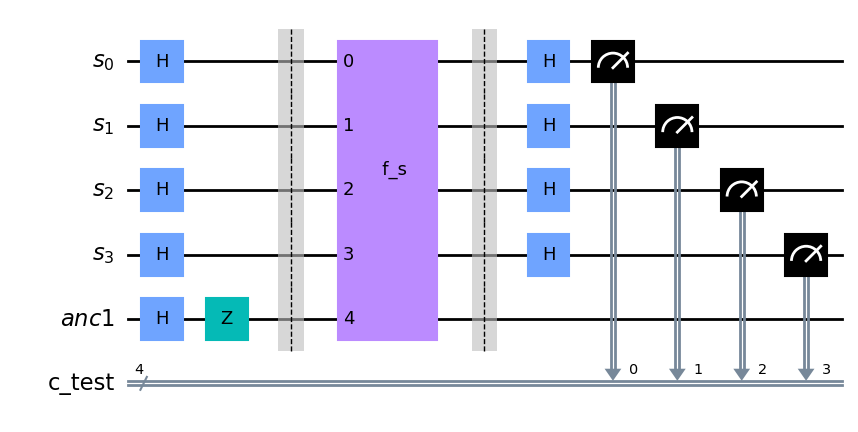
\includegraphics[width=0.8\textwidth]{TFG/imagenes/BV_circuito.png}
    \caption{Circuito, algoritmo BV para s de longitud 4} 
 \end{figure}

 Detallemos brevemente los elementos principales de este circuito:
 \begin{itemize}
     \item \textbf{Qubits}: Se representan en las primeras lineas, cada uno en una línea distinta. El circuito de la figura 2.1 se compone de 5 qubits. Entre ellos vemos un qubit llamado anc1, que es un qubit ancilla, auxiliar. Muchas veces este qubit extra almacenará el resultado de las operaciones, ya que nunca deberíamos modificar los datos originales. Se debe seguir el siguiente esquema: \newline
     
     \begin{center}$\Qcircuit @C=1em @R=.7em {\lstick{|x\rangle}&  \multigate{1}{U_{f}} &\qw & \rstick{|x\rangle}\\ \lstick{|y\rangle} &\ghost{U_{f}} & \qw & \rstick{|y \oplus f(x)\rangle}}$ \end{center}
     
     \item \textbf{Bits clásicos}: Se representan en la ultima fila, todos juntos. Podemos ver el número, en este caso 4, que nos indica el número de bits clásicos que tenemos.
     \item \textbf{Puertas para un qubit}: Podemos observar puertas ya conocidas como Hadamar, Z o la medición que vemos como cae hacia el cable de bits clásicos indicando en que bit se registra la medición.
     \item \textbf{Puerta $f_{s}$}: Como ya mencionamos anteriormente puede haber puertas que se apliquen a varios qubits, en este caso tenemos la puerta, o bloque, que replica la función del problema de Bernstein-Vazirani. Dentro de esta puerta tenemos puertas más pequeñas como las presentadas anteriormente en este mismo apartado. En particular, $f_{s}$ tiene puertas CNOT. En diversos algoritmos, se representa esta puerta como un bloque debido a que la podemos entender como un oráculo, del que no sabemos como funciona internamente.
     \item \textbf{Barreras}: Nos sirven como apoyo para visualizar el algoritmo y poder separar en secciones.
 \end{itemize}

 Para producir este circuito se puede hacer de distintas maneras, ya sea programando en python con apoyo de qiskit o directamente en IBM es posible poner las cajas de los operadores en los qubits que nos interesan.
 
\subsection{Simulaciones y ruido} 
 Una vez que ya hemos visto las puertas que podemos usar en un circuito cuántico, así como un ejemplo del mismo, veamos una introducción a las distintas opciones para la ejecución, utilizaremos las dos siguientes: (qiskit, intro cuantica)
 
 \begin{itemize}
     \item \textbf{Simulación}, en nuestro caso con los simuladores de IBM. Esta posibilidad nos va a ofrecer una simulación teórica de lo que ocurre en nuestro circuito. Será ejecutado a través de un simulador de IBM y nos va a permitir obtener resultados con seguridad y sin ningún problema asociado de errores o ruido.
     \item \textbf{Ordenador cuántico}, utilizaremos los ordenadores de IBM. La tecnología para la creación de ordenadores cuánticos más fieles sigue avanzando. Esta intenta mitigar los errores que tiene cada operación, así como los errores relacionados con el ruido del entorno que influyen en el estado del sistema modificándolo. Cada ordenador tiene su propia estructura y sus estudios sobre los errores que se cometen en cada qubit, así como calibraciones. Se puede ver en la figura 2.2, los errores de cada qubit así como la estructura del ordenador. Qiskit analizará el circuito y lo adaptará a la arquitectura del sistema elegido para minimizar los errores.
 \end{itemize}

 Ambas opciones utilizan el mismo mecanismo, repiten el proceso tantas veces como les sea requerido y muestran la frecuencia acumulada de los resultados (mediciones) o directamente las probabilidades sobre el número total de ejecuciones.

 
 \begin{figure}[H]
    \centering
    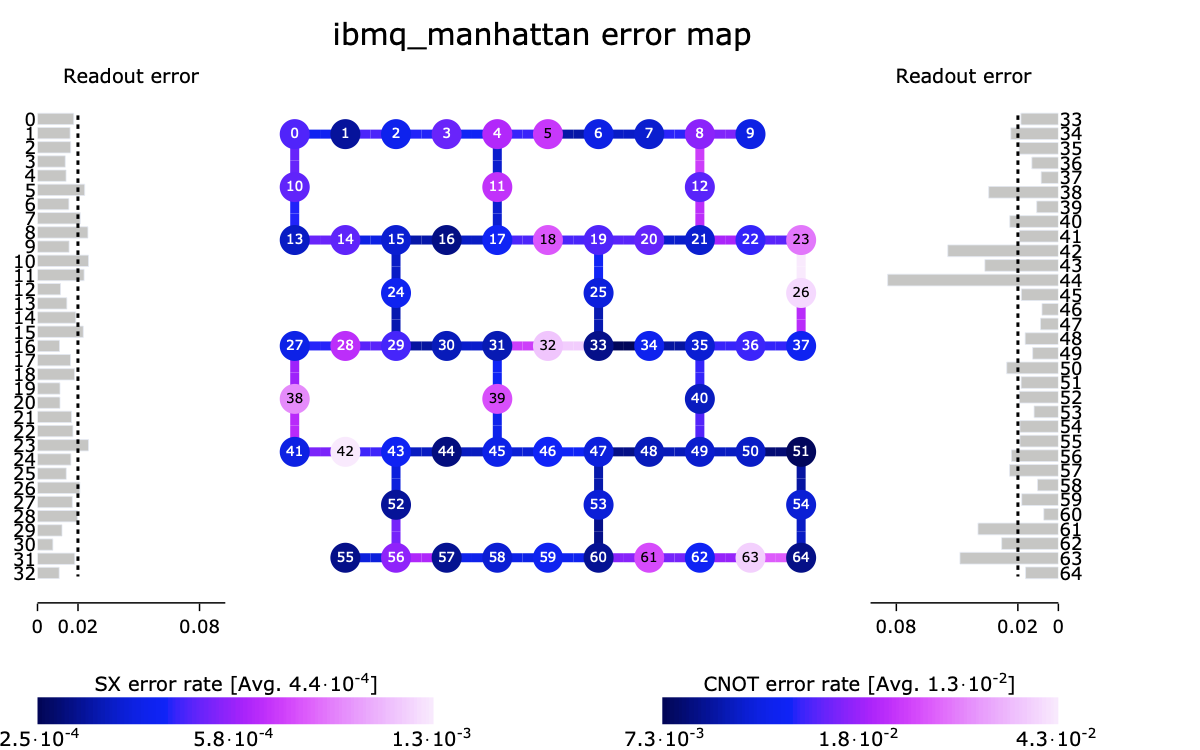
\includegraphics[width=\textwidth]{TFG/imagenes/system_error_manhattan.png}
    \caption{Mapa de errores del ibmq\_manhattan} 
 \end{figure}
 
 \vspace{5pt}
 
 Veamos un ejemplo para entender la diferencia de resultados de utilizar un opción u otra. Para ello vamos a usar los resultados del circuito presentado en la figura 2.1 del algoritmo de Bernstein-Vazirani que se presentará en el siguiente capítulo. Este algoritmo nos debería dar un resultado único, pero veamos lo que ocurre. \newline

 \begin{figure}[H]
    \centering
    \begin{subfigure}[H]{0.48\textwidth}
        \centering
        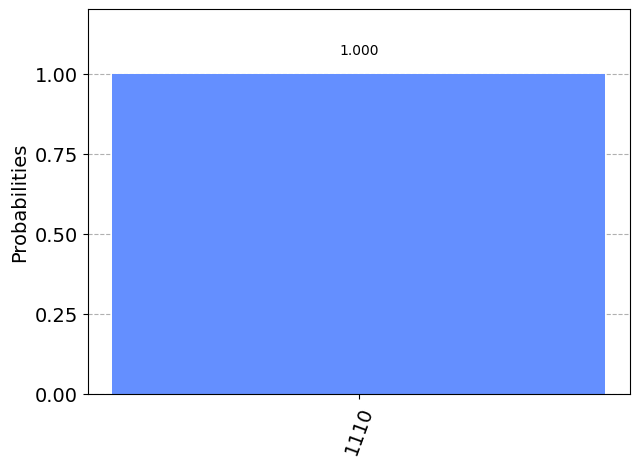
\includegraphics[width=\textwidth]{TFG/imagenes/BV_simulación.png}
        \caption{Simulación}
    \end{subfigure}
    \hfill
    \begin{subfigure}[H]{0.48\textwidth}
        \centering
        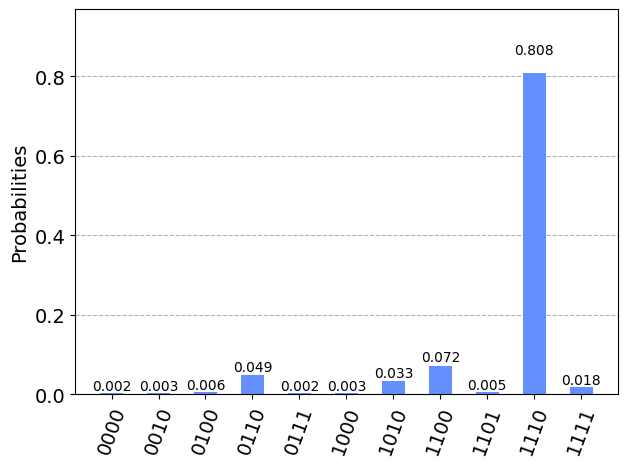
\includegraphics[width=\textwidth]{TFG/imagenes/BV_ruido.png}
        \caption{Sistema cuántico}
    \end{subfigure}
        \caption{Diferencias en resultados de ejecución del algoritmo de Bernstein-Vazirani}
 \end{figure}
\vspace{5pt}

Se puede observar en la figura 2.3 la diferencia entre la simulación teórica (a) y la ejecución con el sistema ibmq\_quito (b). Nuestra simulación nos ha dado únicamente el resultado querido, pero al ejecutarlo en sistema cuántico nos ha dado una variedad de resultados, aunque no todos los posibles. Si bien es cierto que el más probable, con suficiente diferencia, es idéntico al obtenido con la simulación. Cabe destacar de la figura 2.3.b que los de mayor probabilidad, una vez eliminada la solución, son aquellos en los cuales solo varía 1 dígito y por el contrario, el complementario binario no ha aparecido como resultado en todas las ejecuciones realizadas.

\section{Propiedades Metamórficas / Testing metamórfico}

Informalmente entendemos como propiedad metamórfica aquella que podemos derivar de forma lógica de una definición o especificación. Empecemos con un ejemplo para ponernos en situación, nos vamos a fijar en la función seno, $f(x)=sin(x)$.\newline

La definición que aprendemos cuando empezamos a ver trigonometría es que el seno es la proporción entre el cateto opuesto y la hipotenusa en un triángulo rectángulo. Teniendo esta imagen la cabeza es muy fácil darse cuenta que $sin(x)=sin(x + 2\pi)=sin(\pi-x)$. Estas son dos propiedades metamórficas de la función seno. \newline

Veamos ahora que es lo que consideramos formalmente una regla o propiedad metamórfica y como llegamos a los pasos de testing metamórfico: (Metamorfic testing paper)

\begin{itemize}
    \item \textbf{Relación metamórfica}, PM: Sea $f: X \rightarrow Y$ una función o algoritmo. Se considera que $\mathscr{R} \subseteq X^{n} \times Y^{n}$ es una \textbf{\textit{regla metamórfica}} si es una relación entre una secuencia de entrada $\langle x_{1},x_{2},...,x_{n}\rangle$ con $n>1$ y sus salidas correspondientes $\langle f(x_{1}),f(x_{2}),...,f(x_{n})\rangle$, la cual se puede deducir de forma lógica desde el algoritmo. Es decir, es una propiedad necesaria de f.
    \item \textbf{Entrada original/seguimiento}: Sea $\mathscr{R}$ una relación metamórfica y sea $\langle x_{1},x_{2},...,x_{k}\rangle$ la secuencia original con sus respectivos resultados. Denotaremos como \textbf{\textit{entrada original}}, source input, a   $\langle x_{1},x_{2},...,x_{k}\rangle$  los cuales son datos definidos o caracterizados, es decir, ya conocidos. A su vez, podemos generar $\langle x_{k+1},x_{k+2},...,x_{n}\rangle$, los cuales están construidos en base a la entrada original e incluso a la salida de esta. A esta secuencia la llamaremos \textbf{\textit{entrada de seguimiento}}, o en inglés follow-up input.
    \item \textbf{Grupo metamórfico de entrada}: Llamaremos \textbf{\textit{grupo metamórfico de entrada}} a la secuencia definida por la entrada original y la de seguimiento, es decir, $\langle x_{1},x_{2},...,x_{k},x_{k+1},...,x_{n}\rangle$.
    \item \textbf{Testing metamórfico}, TM: Sea $f$ la función o algoritmo objetivo, $P$ una implementación de $f$ y $\mathscr{R}$ una regla metamórfica de $f$. Para realizar \textbf{\textit{testing metamórfico}} sobre $P$ seguiremos los siguiente pasos:
    \begin{itemize}
        \item Definimos $\mathscr{R}'$ reemplazando $f$ por $P$ en $\mathscr{H}$.
        \item Dado una entrada original, generamos sus salidas según $P$, construimos a partir de estos, los casos de seguimiento $\langle x_{k+1},...,x_{n}\rangle$, y obtenemos $\langle P(x_{k+1}),...,P(x_{n})\rangle$.
        \item Estudiamos los resultados obtenidos respecto a $\mathscr{R}'$. Si no es satisfacible entonces diremos que $P$ no es correcto.
    \end{itemize}
\end{itemize}

La estrategia presentada anteriormente para TM, será la que se siga en la implementación de las propiedades que se obtendrán a lo largo de este documento. \newline

Para finalizar con esta introducción vamos a revisar brevemente un par de ventajas y retos que presenta el camino que estamos tomando para probar la corrección, o más bien la no corrección, de un algoritmo. \newline

\textbf{Ventajas}:
\begin{itemize}
    \item \textbf{Simplicidad}. El concepto e interpretación de una PM es bastante simple en comparación con otros conceptos que se utilizan dentro del campo del testing. Se ha visto en estudios, que incluso gente con poca experiencia, podrían utilizar estas técnicas en relativamente poco tiempo de forma efectiva.(ref 55,73 del paper de testing)
    \item \textbf{Facilidad en la implementación}. Si partimos de la ventaja anterior como es la simplicidad de la definición, podemos continuar que la implementación de este test es prácticamente seguir los pasos explicados en la definición de TM (link a la definicion).
\end{itemize}

\vspace{10pt}

\textbf{Retos}:
\begin{itemize}
    \item \textbf{Generación efectiva de los grupos metamórficos de entrada}. Aun se sigue estudiando que garantías tenemos en la efectividad que puede tener la elección del grupo metamórfico de entrada en la demostración de la corrección de un algoritmo y en particular, la forma en la que obtenemos nuestra entrada original, ya que la entrada de seguimiento la generamos a partir de esta. Al fin y al cabo nuestro objetivo es maximizar la identificación de errores o defectos en $P$.
    \item \textbf{Estructura del TM}. Debido a la juventud de este tipo de testing y la gran variedad de PM, aun no hay un acuerdo sobre una estructura definida y formal que nos proporcione seguridad en nuestra pruebas y englobe a todas las posibilidades que tenemos dentro de las PM. Aunque, si bien es cierto, ya ha ayudado a identificar diversos errores en sistemas muy estudiados con otros métodos de testing, como por ejemplo los compiladores GCC y LLVM de C, en los cuales encontró más de 100 defectos (\textit{faults}). (ref 50,51,78)
\end{itemize}

Los retos de TM pueden ser una buena base para todo el trabajo futuro que se puede realizar en este campo y las posibilidades que este nos puede ofrecer. Trataremos en más profundidad estás posibilidades en el apartado 5.2 de posibles trabajos futuros (link)




\cleardoublepage

\chapter{Algoritmos cuánticos}
\label{Cap3:Algoritmos}

El siguiente paso en este camino hacia la unión entre la computación cuántica y el \textit{testing} metamórfico es la creación de algoritmos o programas cuánticos que nos ayuden a resolver problemas propuestos o avanzar. \newline

Todo el desarrollo de estos algoritmos se pueden encontrar en los libros principales \cite{B:Nielsen:2002}\cite{B:QuantumScientist:2008}. Presentaremos a continuación todos los algoritmos finales que nos permiten obtener nuestros objetivos, si bien es cierto, solo vamos a presentar el camino completo de creación del algoritmo de Deutsch por su simplicidad. Esto se debe a que para alcanzar nuestro objetivo debemos ir haciendo modificaciones y cálculos sobre nuestros algoritmos hasta dar con la combinación correcta de puertas que nos permita resolverlo.\newline

Esta sección va a seguir prácticamente la misma estructura para cada apartado, a excepción de la suma. Empezará con una introducción, seguida de la exposición del problema a resolver. Entonces nos dispondremos a presentar el algoritmo que lo resuelve, o como lo creamos, y las pruebas realizadas. Es necesario recordar que toda la programación realizada sobre estos algoritmos se encuentra en el repositorio de GitHub \url{https://github.com/sinugarc/TFG.git}

\section{Suma}
\label{Sec3.1:Suma}
 Este primer algoritmo nos va a servir como primera toma de contacto con la programación cuántica, las puertas que podemos utilizar y el uso de \textit{Qiskit}. Veamos cual es el problema a resolver:\newline

 \textbf{Problema 1}: Dadas dos cadenas binarias de igual longitud, queremos obtener la suma bit a bit de ambas.\newline

 Esta operación se va a realizar posteriormente y se usará $\oplus$ como notación. La implementación de este problema es muy simple, bastará con incluir tantos bit ancilla como longitud tenga la cadena que almacene el resultado, así nos aseguramos que no se modifiquen los valores originales y bastará con utilizar la puerta $CNOT$ para ir modificando los valores ancilla correspondientes. Dando lugar en los valores ancilla al resultado de la suma bit a bit de ambas cadenas.\newline

 (PONER CIRCUITO)

 \textbf{Problema 2}: Dadas dos cadenas binarias, queremos obtener la suma de ambas, como si estas fueran representación de número naturales.\newline

 (EXPLICAR Y PONER EL PRIMER CIRCUITO PROGRAMADO)

\section{Deutsch}
\label{Sec3.2:Deutsch}

 El algoritmo de Deutsch\cite{B:QuantumScientist:2008} fue propuesto por David Deutsch en 1985, siendo este uno de los primeros algoritmos propuestos y en sí, el que se podría entender como uno de los problema más simples. Sea $f:\{0,1\}\rightarrow\{0,1\}$, diremos que $f$ es \textbf{balanceada} si $f(0)\neq f(1)$ y diremos que es \textbf{constante} si $f(0)=f(1)$. \newline

 \textbf{Problema}: Dada una función $f:\{0,1\}\rightarrow\{0,1\}$ balanceada o constante, la cual no podemos observar su definición. Queremos determinar si esta función es constante o balanceada.\newline

 \textbf{Solución clásica}: Tenemos que evaluar $f$ en ambos valores y comparar las soluciones.\newline

 Veamos ahora que podemos hacer con un ordenador cuántico, ¿seremos capaces de evaluar $f$ una única vez? \newline

 Primero observamos un ejemplo particular y cómo vamos a llevarlo a un circuito cuántico. Sea $f(0)=1$ y $f(1)=0$, buscamos una matriz unitaria que nos permita representarla en un circuito cuántico, aunque tendremos que hacer alguna modificación más. Por ahora lo que obtenemos es,

 \begin{equation*}
     \begin{matrix}
           & \begin{matrix} \textbf{0} & \textbf{1} \end{matrix} \\
         \begin{matrix} \textbf{0} \\ \textbf{1} \end{matrix} & \begin{bmatrix}
             0 & 1 \\
             1 & 0
         \end{bmatrix}
     \end{matrix}
 \end{equation*}

 \vspace{5pt}

 Donde la columna representa la entrada y la fila la salida. Como ya se mencionó al explicar los qubits del circuito (figura 2.2), es importante conservar la entrada y por lo tanto si $U_{f}$ es la caja negra que representa a $f$, nuestro circuito será:

 \vspace{10pt}

 \begin{center}$\Qcircuit @C=1em @R=.7em {\lstick{|x\rangle}&  \multigate{1}{U_{f}} &\qw & \rstick{|x\rangle}\\ \lstick{|y\rangle} &\ghost{U_{f}} & \qw & \rstick{|y \oplus f(x)\rangle}}$ \end{center}

 \vspace{7pt}

 Es más, si aplicáramos $U_{f}$ dos veces obtendríamos la entrada:

 \vspace{10pt}

 \begin{center}$\Qcircuit @C=1em @R=.7em {\lstick{|x\rangle} & \multigate{1}{U_{f}} & \qw & \qw & \ustick{|x\rangle} \qw & \qw & \qw & \multigate{1}{U_{f}} & \qw & \rstick{|x\rangle}\\ \lstick{|y\rangle} & \ghost{U_{f}} & \qw & \qw & \dstick{|y \oplus f(x)\rangle} \qw & \qw & \qw &\ghost{U_{f}} & \qw & \rstick{|y\rangle}}$\end{center}

 \vspace{14pt}

 Esto se debe a que $f(x)\oplus f(x) = 0$. Pero claro, ¿qué matriz realmente representa a $U_{f}$? Veamos como quedaría respecto a la base:

 \vspace{5pt}
 \begin{center}
 \begin{blockarray}{ccccc}
         & $\mathbf{|00\rangle}$ & $\mathbf{|01\rangle}$ & $\mathbf{|10\rangle}$ & $\mathbf{|11\rangle}$\\
    \begin{block}{c[cccc]}
        $\mathbf{|00\rangle}$ & 0 & 1 & 0 & 0 \\
        $\mathbf{|01\rangle}$ & 1 & 0 & 0 & 0 \\
        $\mathbf{|10\rangle}$ & 0 & 0 & 1 & 0 \\
        $\mathbf{|11\rangle}$ & 0 & 0 & 0 & 1
     \end{block}
\end{blockarray}
\end{center}

\vspace{5pt}

Se podría comprobar que esta matriz es su propia adjunta, por lo que es invertible y unitaria. Por lo que cumple las características necesarias para ser una puerta de un circuito cuántico.\newline

 Ahora que ya tenemos la caja negra deseada, determinada por una matriz unitaria, nos queremos poner a resolver el problema. Como comenté en la introducción de este capítulo, esta va a ser el único algoritmo al que le vamos a seguir la pista de razonamiento de principio a final, es decir, partiremos de una idea inicial y acabaremos en el algoritmo de Deutsch que resuelve este problema.\newline

 Nuestro objetivo es mejorar la complejidad de la solución del problema respecto a la solución clásica. Recordamos que necesitamos evaluar $f$ dos veces, por lo que nuestro objetivo va a ser obtener el resultado evaluando $f$ una única vez. Para ello nos vamos a sustentar en la superposición, para así analizar que ocurre en el $|0\rangle$ y en el $|1\rangle$ al mismo tiempo, es decir, vamos a tener que utilizar la puerta de Hadamard. \newline
 
 \textbf{Primer intento}: Tomamos nuestro primer \textit{input} para el problema, por ejemplo $|x\rangle=|0\rangle$ e $|y\rangle=|0\rangle$ y creamos el primer circuito:

 \vspace{5pt}

 \begin{center}$\Qcircuit @C=1.5em @R=.7em {\lstick{|0\rangle} & \qw & \gate{H} & \qw &\multigate{1}{U_{f}} & \qw & \qw & \qw  \\ \lstick{|0\rangle} & \dstick{\begin{matrix} \Uparrow \\ |\varphi_{0}\rangle \end{matrix}} \qw & \qw  & \dstick{\begin{matrix} \Uparrow \\ |\varphi_{1}\rangle \end{matrix}} \qw & \ghost{U_{f}} & \dstick{\begin{matrix} \Uparrow \\ |\varphi_{2}\rangle \end{matrix}} \qw & \meter & \qw \\}$\end{center}

\vspace{30pt}

Donde cada $\varphi_{i}$ va a representar el estado del sistema en cada momento, esto nos va a ayudar a analizar de forma determinista lo que ocurre en nuestro circuito.\newline

Podemos resumir el circuito como  $U_{f}(H\otimesI)|0,0\rangle$, veamos ahora que estados tenemos en cada instante $i$:

\begin{itemize}
    \item $\mathbf{|\varphi_{0}\rangle} = |0\rangle \otimes |0\rangle = |0,0\rangle$

    \item $\mathbf{|\varphi_{1}\rangle} = (H\otimes I)|0,0\rangle = \left[ \dfrac{|0\rangle + |1\rangle}{\sqrt{2}}\right] |0\rangle = \dfrac{|0,0\rangle+|1,0\rangle}{\sqrt{2}}$

    \item  $\mathbf{|\varphi_{2}\rangle} = \dfrac{|0,f(0)\rangle+|1,f(1)\rangle}{\sqrt{2}}$
\end{itemize}

Si nos fijamos en el ejemplo que expuesto al principio del algoritmo obtendríamos el siguiente estado antes de la medición:

\begin{equation}
    |\varphi_{2}\rangle=\begin{bmatrix}
        0 & 1 & 0 & 0 \\
        1 & 0 & 0 & 0 \\
        0 & 0 & 1 & 0 \\
        0 & 0 & 0 & 1
    \end{bmatrix}
    \begin{bmatrix}
        \frac{1}{\sqrt{2}} \\ 0 \\ \frac{1}{\sqrt{2}} \\ 0 
    \end{bmatrix} = 
    \begin{bmatrix}
        0 \\ \frac{1}{\sqrt{2}} \\ \frac{1}{\sqrt{2}} \\ 0 
    \end{bmatrix} = \dfrac{|0,1\rangle + |1,0\rangle}{\sqrt{2}}
\end{equation}

De aquí podemos observar, que sin importar donde hagamos la medición, el resultado no va a ser concluyente, porque vamos a tener una probabilidad de 0.5 de obtener $|0\rangle$ o $|1\rangle$. Es decir, este primer intento no nos sirve para nuestro objetivo. \newline

\textbf{Segundo intento}: Veamos ahora que ocurre si en vez de poner en superposición el primer qubit, ahora ponemos el segundo, tomando $|1\rangle$ como \textit{input}:

 \vspace{5pt}

 \begin{center}$\Qcircuit @C=1.5em @R=.7em {\lstick{|x\rangle} & \qw & \qw & \qw &\multigate{1}{U_{f}} & \qw & \qw & \qw  \\ \lstick{|1\rangle} & \dstick{\begin{matrix} \Uparrow \\ |\varphi_{0}\rangle \end{matrix}} \qw & \gate{H}  & \dstick{\begin{matrix} \Uparrow \\ |\varphi_{1}\rangle \end{matrix}} \qw & \ghost{U_{f}} & \dstick{\begin{matrix} \Uparrow \\ |\varphi_{2}\rangle \end{matrix}} \qw & \meter & \qw \\}$\end{center}

\vspace{30pt}

Ahora iremos directamente a $|\varphi_{2}\rangle$ :

\begin{equation}
    |\varphi_{2}\rangle=|x\rangle \left[ \dfrac{|0\otimes f(x)\rangle - |1\otimes f(x)\rangle}{\sqrt{2}} \right] = \begin{cases} |x\rangle \:  \left[ \dfrac{|0\rangle-|1\rangle}{\sqrt{2}}\right] \;\; si \: f(x) = 0 \\ \\ |x\rangle \: \left[ \dfrac{|0\rangle-|1\rangle}{\sqrt{2}} \right] \;\; si \: f(x) = 1 \end{cases}
\end{equation}\newline

Esto lo podemo resumir como:

\begin{equation}
    |\varphi_{2}\rangle = (-1)^{f(x)} \;|x\rangle \; \left[ \dfrac{|0\rangle-|1\rangle}{\sqrt{2}}\right]
\end{equation}\newline

Pero al igual que en intento anterior, al intentar medir en cualquiera de ambos qubits no obtendríamos ningún resultado concluyente. Esto nos va a llevar al último intento.\newline

\textbf{Tercer intento}, \textbf{Algoritmo de Deutsch}: Al no ser capaces de obtener un resultado poniendo sólo un qubit en superposición, esta vez vamos a poner ambos en estado de superposición, con  el \textit{input} $|0,1\rangle$. Además, vamos a medir sobre el qubit superior tras aplicar una puerta de Hadamard, que recordamos es su propia inversa. Este es el circuito final que representa al algoritmo de Deutsch:

 \vspace{5pt}

 \begin{center}$\Qcircuit @C=1.5em @R=.7em {\lstick{|0\rangle} & \qw & \gate{H} & \qw &\multigate{1}{U_{f}} & \qw & \gate{H} & \qw & \meter & \qw  \\ \lstick{|1\rangle} & \dstick{\begin{matrix} \Uparrow \\ |\varphi_{0}\rangle \end{matrix}} \qw & \gate{H}  & \dstick{\begin{matrix} \Uparrow \\ |\varphi_{1}\rangle \end{matrix}} \qw & \ghost{U_{f}} & \dstick{\begin{matrix} \Uparrow \\ |\varphi_{2}\rangle \end{matrix}} \qw & \qw & \dstick{\begin{matrix} \Uparrow \\ |\varphi_{3}\rangle \end{matrix}} \qw & \qw & \qw }$\end{center}

\vspace{30pt}

Esto matricialmente nos queda como $(H\otimes I)\:U_{f}\:(H\otimes H)\:|0,1\rangle$ .\newline

Analizamos ahora todos los estados $|\varphi_{i}\rangle$:

\begin{itemize}
    \item $\mathbf{|\varphi_{0}\rangle} = |0\rangle \otimes |1\rangle = |0,1\rangle$

    \vspace{5pt}

    \item  $\mathbf{|\varphi_{1}\rangle} = \left[ \dfrac{|0\rangle + |1\rangle}{\sqrt{2}}\right] \left[ \dfrac{|0\rangle - |1\rangle}{\sqrt{2}}\right]$

    \vspace{5pt}

    \item $\mathbf{|\varphi_{2}\rangle} = \left[ \dfrac{(-1)^{f(0)}\:|0\rangle + (-1)^{f(1)}\:|1\rangle}{\sqrt{2}}\right] \left[ \dfrac{|0\rangle - |1\rangle}{\sqrt{2}}\right]$\newline 
    
    Hemos obtenido este resultado substituyendo $|x\rangle$ en el la ecuación 3.3 (link). Pero veamos que ocurre separando $(-1)^{f(0)}\:|0\rangle + (-1)^{f(1)}\:|1\rangle$ según nuestras posibilidades:
    \begin{itemize}
        \item $f$ es constante: $\dfrac{(-1)^{f(0)}\:|0\rangle + (-1)^{f(1)}\:|1\rangle}{\sqrt{2}} = (\pm 1)\left[ \dfrac{|0\rangle - |1\rangle}{\sqrt{2}}\right]$

        \vspace{5pt}
        
        \item $f$ es balanceada: $\dfrac{(-1)^{f(0)}\:|0\rangle + (-1)^{f(1)}\:|1\rangle}{\sqrt{2}} = (\pm 1)\left[ \dfrac{|0\rangle + |1\rangle}{\sqrt{2}}\right]$

    \end{itemize}

    \vspace{5pt}
    
    \item Y por último obtenemos:
    \begin{equation}\mathbf{|\varphi_{3}\rangle} = \begin{cases} (\pm 1)\:|0\rangle \left[ \dfrac{|0\rangle - |1\rangle}{\sqrt{2}}\right] \;\; si \: f(x)\:\text{es constante} \\ \\ (\pm 1)\:|1\rangle \left[ \dfrac{|0\rangle - |1\rangle}{\sqrt{2}}\right] \;\; si \: f(x)\:\text{es balanceada} \end{cases}\end{equation}
\end{itemize}

Por lo que hemos conseguido nuestro objetivo. Tras una única evaluación de $f$ según la medición del primer qubit, sabremos si $f$ es constante con medición $|0\rangle$ o balanceada, $|1\rangle$. Consiguiendo así nuestro objetivo.\newline

\section{Deutsch-Jozsa}
\label{Sec3.3:Deutsch-Jozsa}
 El algoritmo de Deutsch-Jozsa\cite{B:QuantumScientist:2008} es una generalización del algoritmo de Deutsch del apartado anterior, pero ahora trabajamos con $f:\{0,1\}^{n} \rightarrow\{0,1\}$. El domino se puede entender como los números escrito en binario de 0 a $2^{n}-1$. En este caso vamos a redefinir los conceptos anteriores:

 \begin{itemize}
     \item Diremos que $f$ es \textbf{constante} si todo el domino va a 0 ó a 1.
     \item Diremos que $f$ es \textbf{balanceada} si exactamente la mitad del domino va a 0 y la otra mitad va a 1.
 \end{itemize}

 \textbf{Problema}\label{P:DJ}: Dada una función $f:\{0,1\}^{n} \rightarrow\{0,1\}$ balanceada o constante, la cual no podemos observar su definición. Queremos determinar si esta función es constante o balanceada.\newline

 \textbf{Solución clásica}: Vamos a tener que evaluar la función $f$ tantas veces como sea necesario. El mejor caso es tras 2 ejecuciones, ya que puede darse la situación en la que es balanceada y cada ejecución da un resultado diferente. Por otra parte, el peor caso se da con $2^{n-1}+1$ ejecuciones, ya que si las primeras $2^{n-1}$ son iguales, la siguiente nos va a determinar si es constante o balanceada. Todo esto se debe a que como hipótesis tenemos que es una de las 2 cosas. \newline

 Vamos a partir del circuito inicial, donde $U_{f}$ determina la función $f$:

 \vspace{10pt}

 \begin{center}$\Qcircuit @C=1.5em @R=1em {\lstick{|\mathbf{x}\rangle}& \qw {/^{n}} & \multigate{1}{U_{f}} & \qw {/^{n}} &\qw & \rstick{|\mathbf{x}\rangle}\\ \lstick{|y\rangle} & \qw &\ghost{U_{f}} & \qw & \qw & \rstick{|y \oplus f(\mathbf{x})\rangle}}$ \end{center}

 \vspace{7pt}

 Hay que destacar que $|\mathbf{x}\rangle=|x_{0}x_{1}...x_{n-1}\rangle$, por eso posteriormente escribimos $/^{n}$, para indicar que son n qubits.\newline

 \textbf{Algoritmo de Deutsch-Jozsa\label{A:DJ}}:

 \vspace{10pt}

 \begin{center}$\Qcircuit @C=1.5em @R=1em {
 \lstick{|\mathbf{0}\rangle}& \qw {/^{n}} & \gate{H^{\otimes n}} & \qw {/^{n}} & \multigate{1}{U_{f}} & \qw {/^{n}} & \gate{H^{\otimes n}} & \qw {/^{n}} & \meter & \qw \\ \lstick{|1\rangle} & \dstick{\begin{matrix} \Uparrow \\ |\varphi_{0}\rangle \end{matrix}} \qw & \gate{H} & \dstick{\begin{matrix} \Uparrow \\ |\varphi_{1}\rangle \end{matrix}} \qw &\ghost{U_{f}} & \dstick{\begin{matrix} \Uparrow \\ |\varphi_{2}\rangle \end{matrix}} \qw & \qw & \dstick{\begin{matrix} \Uparrow \\ |\varphi_{3}\rangle \end{matrix}} \qw  & \qw & \qw}$ \end{center}

 \vspace{30pt}

 Que en término de matrices es: $(H^{\otimes n} \otimes I)\:U_{f}\:(H^{\otimes n} \otimes H)\:|\mathbf{0},1\rangle$ \newline

 Antes de analizar los estados en cada $|\varphi_{i}\rangle$, vamos a estudiar que ocurre cuando tenemos la puerta $H^{\otimes n}$ y como se comporta sobre los diferentes estados, así como la notación que utilizamos, ya que esta será necesaria en el análisis de los $|\varphi_{i}\rangle$. \newline

 El estudio sobre las características de $H^{\otimes n}$ se pueden estudiar en profundidad en \citealp[\textit{Quantum computing for computer scientists}]{B:QuantumScientist:2008}, aquí resumiremos los resultados principales que nos van a permitir profundizar en los circuitos cuánticos, ya que la aplicación de esta puerta es muy común.\newline

 Antes de meternos en $H^{\otimes n}$, vamos a definir un producto interno en $\mathbb{Z}_{2}$:\newline

 \begin{equation*}
     \langle\:,\:\rangle\::\{0,1\}^{n} \times \{0,1\}^{n} \rightarrow \{0,1\}\end{equation*}

 Si $\mathbf{x}=x_{0}x_{1}...x_{n-1}$ e $\mathbf{y}=y_{0}y_{1}...y_{n-1}$, entonces:

 \begin{equation*}
     \begin{split}
     \langle\mathbf{x},\mathbf{y}\rangle &= \langle x_{0}x_{1}...x_{n-1},y_{0}y_{1}...y_{n-1}\rangle \\ &= (x_{0}\land y_{0})\oplus(x_{1}\land y_{1})\oplus...\oplus(x_{n-1}\land y_{n-1}) \\ &= x_{0}y_{0}\oplus x_{1}y_{1}\oplus ... \oplus x_{n-1}y_{n-1}
     \end{split}
 \end{equation*}

 Donde $\land$ es la operación lógica AND y $\oplus$ la operación lógica XOR.\newline

 También definimos, $\mathbf{x}\oplus\mathbf{y}=x_{0}\oplus y_{0},x_{1}\oplus y_{1},...,x_{n-1}\oplus y_{n-1}$ como la suma binaria bit a bit.\newline

 Con esto obtenemos las siguiente propiedades del producto interno:

 \begin{itemize}
     \item $\langle \mathbf{x} \oplus \mathbf{x}',\mathbf{y}\rangle=\langle \mathbf{x},\mathbf{y}\rangle \oplus \langle \mathbf{x}',\mathbf{y}\rangle$

     \item $\langle \mathbf{x},\mathbf{y} \oplus \mathbf{y}'\rangle=\langle \mathbf{x},\mathbf{y}\rangle \oplus \langle \mathbf{x},\mathbf{y}'\rangle$

     \item $\langle 0\cdot \mathbf{x},\mathbf{y}\rangle=\langle\mathbf{0},\mathbf{y}\rangle=0$

     \item $\langle \mathbf{x}, 0 \cdot \mathbf{y}\rangle=\langle \mathbf{x},\mathbf{0}\rangle=0$
 \end{itemize}

 Una vez definidas estas operaciones y propiedades vamos a poder definir la matriz que caracteriza a $H^{\otimes n}$. Cabe recordar que cada fila y cada columna representa un elemento de la base, que se corresponde con la representación binaria de la fila y la columna desde 0:
 
 \begin{equation}H^{\otimes n} [\mathbf{i},\mathbf{j}] = \dfrac{1}{\sqrt{2^{n}}}(-1)^{\langle\mathbf{i},\mathbf{j}\rangle}\end{equation}

 Desde aquí podemos obtener las 2 expresiones que utilizaremos a continuación:

 \begin{equation}
     H^{\otimes n}|\mathbf{0}\rangle=H^{\otimes n}[-,\mathbf{0}]=\dfrac{1}{\sqrt{2^{n}}}\sum_{\mathbf{x} \in \{0,1\}^{n}} |\mathbf{x}\rangle
 \end{equation}

 \begin{equation}
     H^{\otimes n}|\mathbf{y}\rangle=H^{\otimes n}[-,\mathbf{y}]=\dfrac{1}{\sqrt{2^{n}}}\sum_{\mathbf{x} \in \{0,1\}^{n}} (-1)^{\langle\mathbf{x},\mathbf{y}\rangle}|\mathbf{x}\rangle
 \end{equation}
 
 Ahora ya si que vamos a observar los estados que se producen en los distintos momentos del circuito:

 \begin{itemize}
     \item $\mathbf{|\varphi_{0}\rangle} = |\mathbf{0},1\rangle$

    \vspace{5pt}

    \item  $\mathbf{|\varphi_{1}\rangle} = \left[ \dfrac{\sum_{\mathbf{x} \in \{0,1\}^{n}}|\mathbf{x}\rangle}{\sqrt{2^{n}}}\right] \left[ \dfrac{|0\rangle - |1\rangle}{\sqrt{2}}\right]$

    \vspace{5pt}

    \item $\mathbf{|\varphi_{2}\rangle} =\left[ \dfrac{\sum_{\mathbf{x} \in \{0,1\}^{n}}(-1)^{f(\mathbf{x})}|\mathbf{x}\rangle}{\sqrt{2^{n}}}\right] \left[ \dfrac{|0\rangle - |1\rangle}{\sqrt{2}}\right]$

    \vspace{5pt}

    \item Ahora tenemos que superponer la superposición, pero en este caso no es la inversa ya que se aplica sobre otros estados $|\mathbf{z}\rangle$:

    \begin{equation}
        \begin{split}\mathbf{|\varphi_{3}\rangle} &= \left[ \dfrac{\sum_{\mathbf{x} \in \{0,1\}^{n}}(-1)^{f(\mathbf{x})}\sum_{\mathbf{z} \in \{0,1\}^{n}}(-1)^{\langle\mathbf{z},\mathbf{x}\rangle}|\mathbf{z}\rangle}{2^{n}}\right] \left[ \dfrac{|0\rangle - |1\rangle}{2^{n}}\right] \\ &= \left[ \dfrac{\sum_{\mathbf{x} \in \{0,1\}^{n}}\sum_{\mathbf{z} \in \{0,1\}^{n}}(-1)^{f(\mathbf{x})}(-1)^{\langle\mathbf{z},\mathbf{x}\rangle}|\mathbf{z}\rangle}{2^{n}}\right] \left[ \dfrac{|0\rangle - |1\rangle}{2^{n}}\right] \\ &= \left[ \dfrac{\sum_{\mathbf{x} \in \{0,1\}^{n}}\sum_{\mathbf{z} \in \{0,1\}^{n}}(-1)^{f(\mathbf{x})\oplus\langle\mathbf{z},\mathbf{x}\rangle}|\mathbf{z}\rangle}{2^{n}}\right] \left[ \dfrac{|0\rangle - |1\rangle}{2^{n}}\right]
        \end{split}
    \end{equation}
 \end{itemize}

 El último paso a analizar y que nos determinará la validez o el que esperamos de este algoritmo es al medición de los primeros n-qubits. Otra manera de estudiar la medición es directamente preguntarnos cual es la probabilidad de que $|\varphi_{3}\rangle$ colapse a $|\mathbf{0}\rangle$ al realizar la medición. Esto es análogo a si bien en el algoritmo anterior nos interesaba medir cuando $|\mathbf{z}\rangle=|\mathbf{0}\rangle$, que por las propiedades estudiadas anteriormente $\langle\mathbf{z},\mathbf{x}\rangle=\langle\mathbf{0},\mathbf{x}\rangle=0$. Con este resultado, si volvemos a la ecuación 3.5 (link):

 \begin{equation}
     \mathbf{|\varphi_{3}\rangle}=\left[ \dfrac{\sum_{\mathbf{x} \in \{0,1\}^{n}}(-1)^{f(\mathbf{x})}|\mathbf{0}\rangle}{2^{n}}\right] \left[ \dfrac{|0\rangle - |1\rangle}{\sqrt{2}}\right]
 \end{equation}

 Veamos cual sería el estado del primer qubit dependiendo de de nuestras posibilidades:

 \begin{itemize}
     \item $f$ es constante:  $\dfrac{\sum_{\mathbf{x} \in \{0,1\}^{n}}(-1)^{f(\mathbf{x})}|\mathbf{0}\rangle}{2^{n}}=\dfrac{\sum_{\mathbf{x} \in \{0,1\}^{n}}(-1)^{f(\mathbf{x})}|\mathbf{0}\rangle}{2^{n}}=\dfrac{(\pm1)2^{n}|\mathbf{0}\rangle}{2^{n}}=(\pm1)|\mathbf{0}\rangle$

     \item $f$ es balanceada: 
     $\dfrac{\sum_{\mathbf{x} \in \{0,1\}^{n}}(-1)^{f(\mathbf{x})}|\mathbf{0}\rangle}{2^{n}}=\dfrac{0|\mathbf{0}\rangle}{2^{n}}=0|\mathbf{0}\rangle$
 \end{itemize}

 Por lo que podemos concluir que este algoritmo resuelve nuestro problema con una única evaluación de $f$. Si el resultado es $|\mathbf{0}\rangle$, $f$ es constante y si es otro cualquiera, $f$ es balanceada. \newline

 \textbf{Observación}: Hay que tener en cuenta, que si la función no es ni balanceada ni constante, este algoritmo no soluciona el problema y los resultados no son concluyentes. Esto se debe a que cualquier valor que nos devuelva el algoritmo tiene un interpretación $|\textbf{0}\rangle$ $f$ constante y si no, $f$ es balanceada. Es decir, si tenemos una función $f$ que no es ni constante ni balanceada, el resultado sea el que sea va a ser erróneo. Y esto explica porque es una de nuestras hipótesis. \newline

\textbf{Oráculo}: El oráculo que utilizamos para este algoritmo puede venir de dos sitios distintos. Podemos programarlo con ayuda de qiskit\footnote{\url{https://learn.qiskit.org/course/ch-algorithms/deutsch-jozsa-algorithm}}, ya que nos explica como crear el oráculo de DJ, sea la función balanceada o constante. O bien, una vez definida la función crear la matriz que representa al operador.\newline
 
\textbf{Simulaciones}: En el repositorio podemos encontrar este algoritmo programado con ayuda de \textit{Qiskit}. Una de las peculiaridades que encontramos es la forma en la que \textit{Qiskit} nos presenta los qubits, más bien hay una permutación en la base respecto a la generalmente utilizamos al formalizar matrices. Esto puede ser un problema cuando las puertas las creamos como un operador a partir de la matriz que las determina. El ejemplo de esta situación esta programado (en el test del repositorio), así como pruebas del algoritmo de DJ con la misma matriz. \newline

Si bien es cierto que todos aquellos algoritmos que tiene programado el oráculo con el procedimiento de Qiskit de forma balanceada su resultado es el ket $|\mathbf{1}\rangle$, esto no tiene porque ser cierto. Si recordamos el análisis final del algoritmo, si obtenemos $|\textbf{0}\rangle$ entonces $f$ es constante y si no, $f$ es balanceada. Por lo que si miramos el algoritmo programado con un operador matricial, podemos observar como el resultado no es ni $|\textbf{0}\rangle$, ni $|\textbf{1}\rangle$, si no que obtenemos $|01\rangle$.


\section{Bernstein-Vazirani}
\label{Sec3.4:BV}

El algoritmo de Bernstein-Vazirani, fué presentado por Ethan Bernstein and Umesh Vazirani\cite{AR:BV:1997}. Se puede entender que este algoritmo es una generalización más del algoritmo de Deutsch-Jozsa \footnote{https://learn.qiskit.org/course/ch-algorithms/bernstein-vazirani-algorithm}. \newline

\textbf{Problema}: Sea $f:\{0,1\}^{n} \rightarrow \{0,1\}$, sea $\mathbf{s}=s_{0}s_{1}...s_{n-1}$, por hipótesis $f(\mathbf{x})=\mathbf{s}\cdot \mathbf{x}\: \text{mod}\:2 = s_{0}x_{0} \oplus s_{1}x_{1} \oplus ... \oplus s_{n-1}x_{n-1}$. Queremos obtener la cadena $\mathbf{s}$.\newline

\textbf{Solución clásica}: Ejecutamos la función $f$ $n$ veces una con cada elemento de la base canónica. Esto nos permitirá obtener los $n$ elementos de $\mathbf{s}$.\newline

\textbf{Algoritmo de Bernstein-Vazirani}:

 \vspace{10pt}

 \begin{center}$\Qcircuit @C=1.5em @R=1em {
 \lstick{|\mathbf{0}\rangle}& \qw {/^{n}} & \gate{H^{\otimes n}} & \qw  & \qw {/^{n}} & \multigate{1}{U_{f}} & \qw {/^{n}} & \gate{H^{\otimes n}} & \qw {/^{n}} & \meter & \qw \\ \lstick{|0\rangle} & \dstick{\begin{matrix} \Uparrow \\ |\varphi_{0}\rangle \end{matrix}} \qw & \gate{H} & \gate{Z} & \dstick{\begin{matrix} \Uparrow \\ |\varphi_{1}\rangle \end{matrix}} \qw &\ghost{U_{f}} & \dstick{\begin{matrix} \Uparrow \\ |\varphi_{2}\rangle \end{matrix}} \qw & \qw & \dstick{\begin{matrix} \Uparrow \\ |\varphi_{3}\rangle \end{matrix}} \qw  & \qw & \qw}$ \end{center}

 \vspace{30pt}

 De forma matricial: $(H^{\otimes n} \otimes I)\: U_{f}\:(I\otimes Z)\:(H^{\otimes n} \otimes H) |\mathbf{0},0\rangle$ \newline

 Veamos ahora los estados alcanzados, similares al circuito anterior:

 \begin{itemize}
     \item $\mathbf{|\varphi_{0}\rangle} = |\mathbf{0},0\rangle$

    \vspace{5pt}

    \item  $\mathbf{|\varphi_{1}\rangle} = \left[ \dfrac{\sum_{\mathbf{x} \in \{0,1\}^{n}}|\mathbf{x}\rangle}{\sqrt{2^{n}}}\right] \left[ \dfrac{|0\rangle - |1\rangle}{\sqrt{2}}\right]$

    \vspace{5pt}

    \item Aplicamos las función $f$:
    
    \begin{equation} \label{eq:BV:phi2}
    \mathbf{|\varphi_{2}\rangle} =\left[ \dfrac{\sum_{\mathbf{x} \in \{0,1\}^{n}}(-1)^{f(\mathbf{x})}|\mathbf{x}\rangle}{\sqrt{2^{n}}}\right] \left[ \dfrac{|0\rangle - |1\rangle}{\sqrt{2}}\right]\end{equation}

    \vspace{5pt}

    \item Ahora tenemos que superponer la superposición, aplicada sobre otros estados $|\mathbf{z}\rangle$:

    \begin{equation}\label{eq:BV:phi3}
        \begin{split}\mathbf{|\varphi_{3}\rangle} &= \left[ \dfrac{\sum_{\mathbf{x} \in \{0,1\}^{n}}(-1)^{f(\mathbf{x})}\sum_{\mathbf{z} \in \{0,1\}^{n}}(-1)^{\langle\mathbf{z},\mathbf{x}\rangle}|\mathbf{z}\rangle}{2^{n}}\right] \left[ \dfrac{|0\rangle - |1\rangle}{2^{n}}\right] \\ &= \left[ \dfrac{\sum_{\mathbf{x} \in \{0,1\}^{n}}\sum_{\mathbf{z} \in \{0,1\}^{n}}(-1)^{f(\mathbf{x})}(-1)^{\langle\mathbf{z},\mathbf{x}\rangle}|\mathbf{z}\rangle}{2^{n}}\right] \left[ \dfrac{|0\rangle - |1\rangle}{2^{n}}\right] \\ &= \left[ \dfrac{\sum_{\mathbf{x} \in \{0,1\}^{n}}\sum_{\mathbf{z} \in \{0,1\}^{n}}(-1)^{f(\mathbf{x})\oplus\langle\mathbf{z},\mathbf{x}\rangle}|\mathbf{z}\rangle}{2^{n}}\right] \left[ \dfrac{|0\rangle - |1\rangle}{2^{n}}\right] \\  &= \left[ \dfrac{\sum_{\mathbf{x} \in \{0,1\}^{n}}\sum_{\mathbf{z} \in \{0,1\}^{n}}(-1)^{\langle\mathbf{s},\mathbf{x}\rangle\oplus\langle\mathbf{z},\mathbf{x}\rangle}|\mathbf{z}\rangle}{2^{n}}\right] \left[ \dfrac{|0\rangle - |1\rangle}{2^{n}}\right] \\ &= \left[ \dfrac{\sum_{\mathbf{x} \in \{0,1\}^{n}}\sum_{\mathbf{z} \in \{0,1\}^{n}}(-1)^{\langle\mathbf{s}\oplus \mathbf{z},\mathbf{x}\rangle}|\mathbf{z}\rangle}{2^{n}}\right] \left[ \dfrac{|0\rangle - |1\rangle}{2^{n}}\right] \\
        \end{split}
    \end{equation}
 \end{itemize}

 Veamos que esta ocurriendo en ese primer bloque de qubits, que será al que apliquemos la medición, si bien en el algoritmo anterior nos interesaba medir cuando $|\mathbf{z}\rangle=|\mathbf{0}\rangle$, pero ahora queremos obtener la cadena $\mathbf{s}$, por lo que vamos a ver que sucede cuando $|\mathbf{z}\rangle=|\mathbf{s}\rangle$.

 \begin{equation}
    \dfrac{\sum_{\mathbf{x} \in \{0,1\}^{n}}(-1)^{\langle\mathbf{s}\oplus \mathbf{s},\mathbf{x}\rangle}|\mathbf{s}\rangle}{2^{n}} = \dfrac{\sum_{\mathbf{x} \in \{0,1\}^{n}}(-1)^{\langle\mathbf{0},\mathbf{x}\rangle}|\mathbf{s}\rangle}{2^{n}}= \dfrac{\sum_{\mathbf{x} \in \{0,1\}^{n}}|\mathbf{s}\rangle}{2^{n}} = |\mathbf{s}\rangle
 \end{equation}

 \vspace{5pt}

 ¿Qué está ocurriendo aquí?, lo que hemos observado es que la amplitud de $|\mathbf{s}\rangle$ es 1, y si recordamos la teoría de los sistemas cuánticos, la suma de los cuadrados de las amplitudes es 1. Es decir, las amplitudes del resto de posibles valores de $|\mathbf{z}\rangle$ es 0. Por lo que al hacer la medición sobre el primer bloque de qubits nos devolverá la cadena $\mathbf{s}$ deseada, al ser su probabilidad de aparición 1. Podemos concluir entonces que hemos obtenido la cadena $\mathbf{s}$ con una única ejecución de $f$, mejorando así la solución clásica para este algoritmo.\newline

 
 \textbf{Oráculo}: Antes de presentar las simulaciones realizadas, vamos a estudiar como a partir de una cadena $\mathbf{s}$ podemos construir un oráculo funcione como $f_{s}$. Según el valor en la cadena se ejecuta una puerta y otra. Sí el valor es 0, entonces pondremos una puerta identidad en la linea del qubit de esa posición para indicar que no se hace nada y si el valor es 1, pondremos una puerta CNOT entre el qubit de la posición y el qubit ancilla, donde el qubit de control es el de la posición del valor. Estos ejemplo se pueden encontrar en el archivo de BV sin puertas, la función \textit{$bv\_fgenerator(qc,n0,s)$}, veamos un par de ejemplos ahora:
 
 \begin{figure}[H]
    \centering
    \begin{subfigure}[H]{0.35\textwidth}
        \centering
        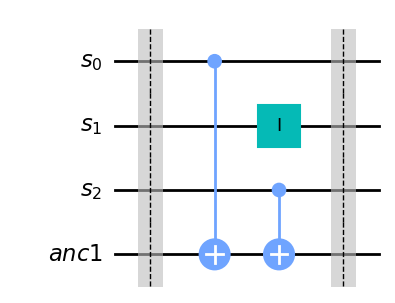
\includegraphics[width=\textwidth]{TFG/imagenes/BVgate1.png}
        \caption{Oráculo para la cadena $\mathbf{s}=101$}
        \label{sFig:BVgate1}
    \end{subfigure}
    \hspace{10pt}
    \begin{subfigure}[H]{0.35\textwidth}
        \centering
        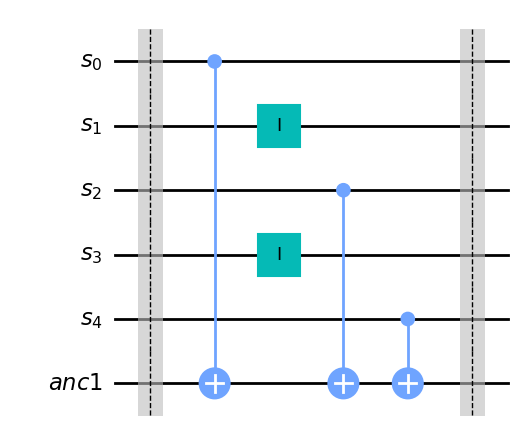
\includegraphics[width=\textwidth]{TFG/imagenes/BVgate2.png}
        \caption{Oráculo para la cadena $\mathbf{s}=10101$}
        \label{sFig:BVgate2}
    \end{subfigure}
        \caption{Ejemplo de oráculos para el algoritmo de BV}
    \label{FIG:BVOraculo}
 \end{figure}


 \textbf{Simulaciones}: Las simulaciones de este algoritmo ya han sido presentadas a lo largo del texto como ejemplo cuando se explicaban las distintas partes de la programación cuántica. Para ampliar estos ejemplos así como revisar el código, se pueden ver en el repositorio.\newline


\section{Simon}
\label{Sec3.5:Simon}
 El algoritmo de Simon, o de periodicidad de Simon, va a ser el primero que no va a usar únicamente computación cuántica, si no que la combina con computación clásica al final del mismo. Veremos cual es el problema y la parte cuántica de la solución, para así ver como procedemos posteriormente hasta encontrar la solución buscada. \newline

 Sea $f:\{0,1\}^{n} \rightarrow\{0,1\}^{n}$, la cual no conocemos su definición, pero si sabemos es periódica en el sentido de que existe una cadena binaria $\mathbf{c}=c_{0}c_{1}...c_{n-1}$ tal que $\forall \mathbf{x},\mathbf{y} \in \{0,1\}^{n}$ entonces, $f(\mathbf{x})=f(\mathbf{y})$ si y solo si $\mathbf{x}=\mathbf{y}\oplus\mathbf{c}$ , donde $\oplus$ es la suma binaria bit a bit. Llamaremos $\mathbf{c}$ al \textbf{periodo} de $f$. \newline

 \textbf{Problema}: Dada una función $f:\{0,1\}^{n} \rightarrow\{0,1\}^{n}$ con periodo $\mathbf{c}=c_{0}c_{1}...c_{n-1}$. Queremos determinar cual es el periodo de $f$ teniendo en cuenta que no conocemos su definición. \newline

 \textbf{Solución clásica}: Vamos ejecutando $f$ hasta encontrar una coincidencia. En el peor de los casos, la función es inyectiva y por lo tanto $\mathbf{c}=|\mathbf{0}\rangle$, para esto habrá que ejecutar $f$ al menos sobre la mitad del dominio, es decir, $2^{n-1}+1$ ejecuciones. Esto se debe a que si existiera un periodo distinto de \textbf{0}, ya habríamos encontrado alguna coincidencia entre la imagen de 2 elementos del dominio.  \newline
 
 Vamos a partir del circuito inicial, donde $U_{f}$ determina la función $f$:

 \vspace{10pt}

 \begin{center}$\Qcircuit @C=1.5em @R=1em {\lstick{|\mathbf{x}\rangle}& \qw {/^{n}} & \multigate{1}{U_{f}} & \qw {/^{n}} &\qw & \rstick{|\mathbf{x}\rangle}\\ \lstick{|\mathbf{y}\rangle} & \qw {/^{n}} &\ghost{U_{f}} & \qw {/^{n}} & \qw & \rstick{|\mathbf{y} \oplus f(\mathbf{x})\rangle}}$ \end{center}

 \vspace{7pt}

 \textbf{Algoritmo de Simon}, parte cuántica:

 \vspace{3pt}

 \begin{center}$\Qcircuit @C=1.5em @R=1em {
 \lstick{|\mathbf{0}\rangle}& \qw {/^{n}} & \gate{H^{\otimes n}} & \qw {/^{n}} & \multigate{1}{U_{f}} & \qw {/^{n}} & \gate{H^{\otimes n}} & \qw {/^{n}} & \meter & \qw \\ \lstick{|\mathbf{0}\rangle} & \dstick{\begin{matrix} \Uparrow \\ |\varphi_{0}\rangle \end{matrix}} \qw & \qw {/^{n}} & \dstick{\begin{matrix} \Uparrow \\ |\varphi_{1}\rangle \end{matrix}} \qw &\ghost{U_{f}} & \dstick{\begin{matrix} \Uparrow \\ |\varphi_{2}\rangle \end{matrix}} \qw & \qw {/^{n}} & \dstick{\begin{matrix} \Uparrow \\ |\varphi_{3}\rangle \end{matrix}} \qw  & \qw & \qw}$ \end{center}

 \vspace{30pt}

 Si lo observamos como operación matricial: $(H^{\otimes n}\otimes I)\:U_{f}\:(H^{\otimes n}\otimes I)\:|\mathbf{0},\mathbf{0}\rangle$\newline

 Análogamente al algoritmo de Deutsch-Jozsa, analizamos los estados del circuito:

 \begin{itemize}
     \item $\mathbf{|\varphi_{0}\rangle} = |\mathbf{0},\mathbf{0}\rangle$

    \vspace{5pt}

    \item  $\mathbf{|\varphi_{1}\rangle} = \dfrac{\sum_{\mathbf{x} \in \{0,1\}^{n}}|\mathbf{x},\mathbf{0}\rangle}{\sqrt{2^{n}}}$

    \vspace{5pt}

    \item $\mathbf{|\varphi_{2}\rangle} = \dfrac{\sum_{\mathbf{x} \in \{0,1\}^{n}}|\mathbf{x},f(\mathbf{x})\rangle}{\sqrt{2^{n}}}$

    \vspace{5pt}
    
    \item $\mathbf{|\varphi_{3}\rangle} =\dfrac{\sum_{\mathbf{x} \in \{0,1\}^{n}}\sum_{\mathbf{z} \in \{0,1\}^{n}}(-1)^{\langle \mathbf{z},\mathbf{x}\rangle}|\mathbf{z},f(\mathbf{x})\rangle}{2^{n}}$

 \end{itemize}

 Si bien antes era algo más directo que nos proporcionaba el resultado, aquí tenemos que analizarlo un poco más, ver hasta donde llega nuestro algoritmo cuántico y que es lo que obtenemos de él. La propiedad principal es la periodicidad de $f$, por lo que por definición  $|\mathbf{z},f(\mathbf{x})\rangle=|\mathbf{z},f(\mathbf{x}\oplus \mathbf{c})\rangle$. Vamos a estudiar el coeficiente al agruparlos, al ser mismo ket:

 \begin{equation}
    \begin{split}
     \dfrac{(-1)^{\langle \mathbf{z},\mathbf{x}\rangle}+(-1)^{\langle \mathbf{z},\mathbf{x}\oplus \mathbf{c}\rangle}}{2} &= \dfrac{(-1)^{\langle \mathbf{z},\mathbf{x}\rangle}+(-1)^{\langle \mathbf{z},\mathbf{x}\rangle \oplus \langle \mathbf{z}, \mathbf{c}\rangle}}{2} \\ &= \dfrac{(-1)^{\langle \mathbf{z},\mathbf{x}\rangle}+(-1)^{\langle \mathbf{z},\mathbf{x}\rangle}(-1)^{\langle \mathbf{z}, \mathbf{c}\rangle}}{2}
    \end{split}
 \end{equation}

 Por lo que si $\langle \mathbf{z}, \mathbf{c}\rangle=1$, entonces los sumandos se cancelan. Por otra parte, si $\langle \mathbf{z}, \mathbf{c}\rangle=0$ el coeficiente será $(\pm 1)$, es decir, al realizar la medición sobre el primer bloque de qubits, solo obtendremos aquellos tales que $\langle \mathbf{z}, \mathbf{c}\rangle=0$.

 \vspace{14pt}

 Pero, ¿proporciona esto una solución esto nuestro algoritmo? Visto así directamente puede parecer que no, debido a que cada vez que lo ejecutemos nos proporcionará una cadena distinta que tiene esa característica. Pero tras obtener n cadenas, obtenemos un sistema de ecuaciones a partir del cual obtenemos la cadena $\mathbf{c}$ deseada. Aquí es donde entraría la computación clásica para acabar de resolver el problema.

 \vspace{14pt}

 Se puede ver la mejora respecto a la solución clásica, ya que al ser todas las cadenas equiprobables, obtendremos $n$ cadenas distintas en menos ejecuciones que $2^{n-1}+1$, para $n$ suficientemente grande. Se puede ver un ejemplo concreto del desarrollo completo del algoritmo con $f:\{0,1\}^{3} \rightarrow\{0,1\}^{3}$ en \textit{Quantum computing for computer scientists, 190}\cite{B:QuantumScientist:2008}.

 \vspace{14pt}

 \textbf{Oráculo}: Debido a su complejidad se importa directamente desde Qiskit.\newline

 \textbf{Simulaciones}: Debido a que utilizamos este circuito, sin ninguna modificación, al comprobar nuestras MR, las simulaciones se encuentran en el \href{https://github.com/rodelanu/TFG/tree/main}{repositorio común}, en el archivo \href{https://github.com/rodelanu/TFG/blob/main/3_Simon_Rules.ipynb}{sobre las reglas del algoritmo de Simon}.

 \vspace{10pt}

 El circuito, análogo al teórico presentado anteriormente, para el algoritmo de Simon, con una cadena $\mathbf{c}$ de longitud 3 es:

 
 \begin{figure}[H]
    \centering
    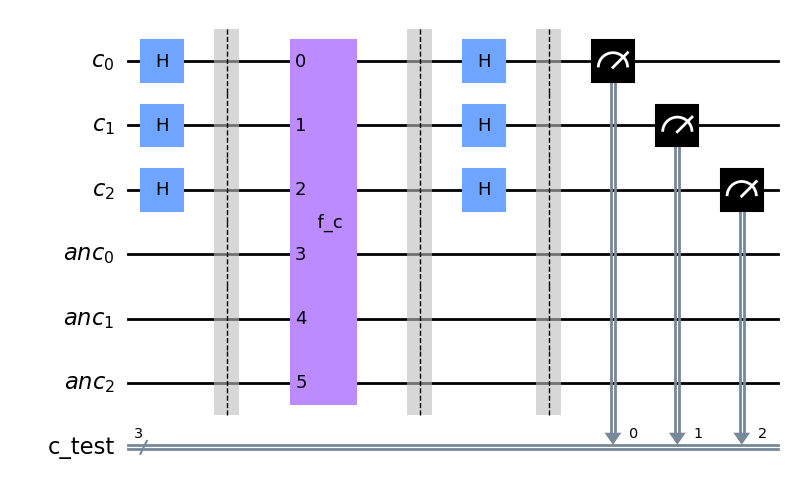
\includegraphics[width=0.7\textwidth]{TFG/imagenes/simon1.png}
    \caption{Circuito, algoritmo Simon con $\mathbf{c}=100$}
    \label{Fig:CircuitoSimon1}
 \end{figure}

 Lo hemos simulado y ejecutado en un sistema cuántico de IBM y estos son los resultados. Además de observar el ruido del sistema cuántico, se va a poder apreciar ambas formas de realizar el histograma, ya sea con conteo o probabilidades.

 \begin{figure}[H]
    \centering
    \begin{subfigure}[H]{0.48\textwidth}
        \centering
        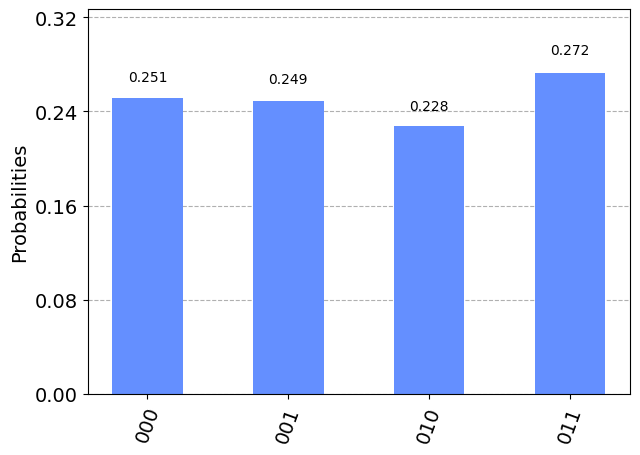
\includegraphics[width=\textwidth]{TFG/imagenes/simonSim.png}
        \caption{Simulador}
        \label{sFig:SimonSim}
    \end{subfigure}
    \hfill
    \begin{subfigure}[H]{0.48\textwidth}
        \centering
        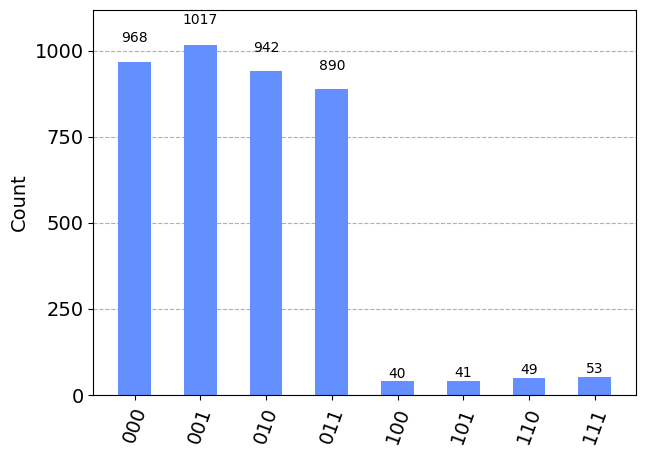
\includegraphics[width=\textwidth]{TFG/imagenes/simonReal.png}
        \caption{Sistema cuántico}
        \label{sFig:SimonIBM}
    \end{subfigure}
        \caption{Resultados del algoritmo Simon para la cadena $\mathbf{c}=100$. }
    \label{FIG:SimonRes}
 \end{figure}
    
\section{Transformada cuántica de Fourier}
\label{Sec3.6:Fourier}

Este apartado va a tratar sobre la transformada cuántica de Fourier, QFT del inglés \textit{Quantum Fourier transform} y una de sus aplicaciones más directas, la estimación cuántica de fase, QPE del inglés \textit{Quantum phase estimation}. Si bien es cierto que todos los algoritmos anteriores tenían un problema a resolver, el estudio de estos algoritmos se basan en la gran utilidad que tienen en cualquier contexto incluida la computación cuántica. Aunque en esta memoria no se tratarán algoritmos o técnicas que necesitan de estos materiales, podemos adelantar que dos de los algoritmos más importantes que se presentan actualmente en programación cuántica lo usan, como por ejemplo el algoritmo de Grover o de búsqueda y el algoritmo de Shor o de factorización.

\subsection{QFT}
Para introducir la transformada de Fourier vamos a ver como se comporta en el caso discreto, ya que nuestra versión cuántica partirá de aquí. 

\subsection{QPE}
 here
\cleardoublepage

\chapter{Propiedades metamórficas}
\label{Cap4:PMetamorficas}

En este último capítulo antes de la conclusión queremos presentar al lector con el objetivo principal de este trabajo. Queremos finalmente unir las propiedades metamórficas con los algoritmos que hemos estudiado en el capítulo \ref{Cap3:Algoritmos}, si bien es cierto solo hemos conseguido estudiar los tres algoritmos que se presentan a continuación. Presentaremos cuales son las propiedades obtenidas, así como de donde las hemos obtenido, para luego pasar a la programación y los circuitos que hemos preparado para poder realizar dichas pruebas.

\section{Deutsch-Jozsa}
\label{Sec4.1:DJ}
En esta sección vamos a estudiar que reglas hemos obtenido del \hyperref[Sec3.3:Deutsch-Jozsa]{algoritmo de Deutsch-Jozsa} y como las hemos implementado en nuestro \href{https://github.com/rodelanu/TFG/blob/main/1_Deutsch_Jozsa_Rules.ipynb}{repositorio}. Recordamos brevemente el problema y el algoritmo obtenido:\newline

\textbf{\hyperref[P:DJ]{Problema}}: Dada una función $f:\{0,1\}^{n} \rightarrow\{0,1\}$ balanceada o constante, la cual no podemos observar su definición. Queremos determinar si esta función es constante o balanceada.\newline

\textbf{\hyperref[A:DJ]{Algoritmo de Deutsch-Jozsa}}:

 \vspace{10pt}

 \begin{center}$\Qcircuit @C=1.5em @R=1em {
 \lstick{|\mathbf{0}\rangle}& \qw {/^{n}} & \gate{H^{\otimes n}} & \qw {/^{n}} & \multigate{1}{U_{f}} & \qw {/^{n}} & \gate{H^{\otimes n}} & \qw {/^{n}} & \meter & \qw \\ \lstick{|1\rangle} & \qw & \gate{H} & \qw &\ghost{U_{f}} & \qw & \qw & \qw  & \qw & \qw}$ \end{center}

 \vspace{30pt}

\textbf{Resultado}: Se obtiene $|\mathbf{0}\rangle$ si $f$ es constante y cualquier otro resultado si $f$ es balanceada.\newline

\textbf{Observación}: No hay que olvidar la importancia de tener como hipótesis que $f$ es constante o balanceada. Pero en este caso, debido a que esta va a formar parte de nuestro \textit{source input}, podemos asegurar esta propiedad. \newline

Suponemos $P$ la implementación del algoritmo de Deutsch-Jozsa a analizar, tal que $P(f)=0$ si $f$ es constante y $P(f)=1$ si $f$ es balanceada., veamos que reglas hemos obtenido y como las vamos a aplicar: \newline


\textbf{Regla I}: Sea $f:\{0,1\}^{n} \rightarrow\{0,1\}$ la función a analizar definida en problema y sea $g : \{0,1\}^{n} -> \{0,1\}^{n}$ un automorfismo. Entonces, $P(f)=|\mathbf{0}\rangle$ si y solo si $P(f\circ g)=|\mathbf{0}\rangle$???? Estudiar a fondo en comparación a lo subido.\newline

\textbf{Regla II}: Sea $f:\{0,1\}^{n} \rightarrow\{0,1\}$ la función a analizar definida en problema y sea $h:\{0,1\}^{n} \rightarrow\{0,1\}$ tal que $h(x) = 1 - f(x)$. Entonces, $P(f)=|\mathbf{0}\rangle$ si y solo si $P(h)=|\mathbf{0}\rangle$. Estudiar si la inversión de 0's y 1's da el mismo ket.

\section{Bernstein-Vazirani}
\label{Sec4.2:BV}
El algoritmo de Bernstein-Vazirani fue el primero presentado como ejemplo al introducir la \hyperref[Sec2.3:Qiskit]{programación cuántica} en el \hyperref[Cap2:Antecedentes]{capítulo 2}. Recapitulemos lo visto cuando se estudió el \hyperref[Sec3.4:BV]{algoritmo de BV}.\newline

\textbf{Problema}: Sea $f:\{0,1\}^{n} \rightarrow \{0,1\}$, sea $\mathbf{s}=s_{0}s_{1}...s_{n-1}$, por hipótesis sabemos que $ f(\mathbf{x})=(\mathbf{s}\cdot \mathbf{x})\: \text{mod}\:2 = s_{0}x_{0} \oplus s_{1}x_{1} \oplus ... \oplus s_{n-1}x_{n-1}$. Queremos obtener la cadena $\mathbf{s}$.\newline

\textbf{Algoritmo de Bernstein-Vazirani}:

 \vspace{10pt}

 \begin{center}$\Qcircuit @C=1.5em @R=1em {
 \lstick{|\mathbf{0}\rangle}& \qw {/^{n}} & \gate{H^{\otimes n}} & \qw  & \qw {/^{n}} & \multigate{1}{U_{f}} & \qw {/^{n}} & \gate{H^{\otimes n}} & \qw {/^{n}} & \meter & \qw \\ \lstick{|0\rangle} & \qw & \gate{H} & \gate{Z} & \qw &\ghost{U_{f}} & \qw & \qw & \qw  & \qw & \qw}$ \end{center}

 \vspace{30pt}

 \textbf{Resultado}: Obtenemos la cadena $|\mathbf{s}\rangle$ en la medición.\newline

 \textbf{Oráculo}: Antes de presentar las reglas y ver su programación, vamos a estudiar como a partir de una cadena $\mathbf{s}$ podemos construir un oráculo funcione como $f_{s}$. \newline

 (FALTA LA INF DEL ORACULO)\newline

 Si suponemos que P es una implementación del algoritmo de BV, vamos a estudiar la reglas obtenidas: \newline

 \textbf{Regla I}\label{R:BV:1}: Sea $\mathbf{s}$ una cadena binaria de longitud $n$ y sea $\mathbf{\Bar{s}}$ su complementario binario. Entonces $P(\mathbf{s})\oplus P(\mathbf{\Bar{s}})=|\mathbf{1}\rangle$ de longitud $n$.\newline

 Esta regla se ha obtenido como un caso particular de la regla general que se presentará a continuación. Ahora bien, ¿Es trascendente el particularizar una regla ya obtenida? Hagamos un pequeño inciso para aclarar este tema.\newline

 La respuesta a esta pregunta es sí, ya que aunque una regla más general cubre muchos más casos, pero eso no nos asegura que encontrar un fallo sea más fácil, por el contrario, puede ser incluso más complejo programar un regla general. Es cierto que este caso es muy simple, aunque la comprobación para este caso es directa, ya que queremos obtener el ket $|\mathbf{1}\rangle$. \newline

 El ejemplo básico que se usa para explicar esta diferencia es el siguiente \cite{AR:MTmain:2008}:\newline

Suponemos que tenemos una implementación $P$ con una MR tal que $f(k\times x)=k\times f(x)$, donde $k \in \mathbb{Z} \setminus \{0\}$. De esta manera se puede extrapolar fácilmente de un \textit{source input} a infinitos casos al fijar un $x$ y variar $k in \mathbb{N}$. Pero en realidad sigue dejando muchísimos casos sin comprobar y tiene cierta dificultad para confirmar todos los \textit{follow-up inputs} en $P$, debido a la cantidad de comprobaciones a realizar para un mismo \textit{source input}. Por otra parte, si tomamos $k=-1$ tenemos otra MR, que aún siendo más débil que la anterior es más fácil de verificar. Y evidentemente, cualquier fallo que se dé con $f(-x)=-f(x)$ es tan efectivo como uno encontrado con la regla general.\newline

Ahora volvamos a nuestra regla I. Para programar este test, vamos a ejecutar por separado $P$ para cada cadena $\mathbf{s}$ y $\mathbf{\Bar{s}}$ y realizaremos la \hyperref[Sec3.1:Suma]{suma} de los resultados antes de realizar la medición. Se podría interpelar que la suma puede dar fallos a la hora de probar la corrección, es decir, que si detectamos un fallo este no sea de $P$, si no de la suma realizada a continuación. A partir de ahora supondremos que la suma cuántica es correcta, es más, tras el artículo \textit{Metamorphic testing of oracle quantum programs}\cite{metamorphicAdd:2022} podemos decir que ha sido incluso probada con el uso de estas mismas técnicas. \newline

El circuito obtenido sería: \newline

 (FALTA IMAGEN DEL CIRCUITO)\newline

La razón por la que esperamos el ket $|\mathbf{1}\rangle$ se debe a que si uno es el complementario binario del otro, su suma binaria es 1 en cada posición.\newline

\textbf{Regla II}: Sean $\mathbf{s}$ y $\mathbf{s}'$ cadenas binarias de longitud $n$. Entonces $P(\mathbf{s})\oplus P(\mathbf{s}')=\mathbf{s} \oplus \mathbf{s}'$.\newline

 Se puede entender que esta es la generalización de la \hyperref[R:BV:1]{regla I}, si bien es cierto podría incluso generalizarse para 2 cadenas que no tengan que tener la misma longitud o incluso se podría interpretar como $P(f_{\mathbf{s}
}\oplus f_{\mathbf{s}'})=P(f_{\mathbf{s}})\oplus P(f_{\mathbf{s}'})$, relacionando así dos \textit{output} del \textit{source input} con uno del \textit{follow-up input}.\newline

 Las reglas anteriores han sido obtenidas de forma directa por la naturaleza del problema, donde si el resultado es la cadena con la que hemos generado el oráculo, entonces la suma binaria se debe conservar tanto en el \textit{source input} como en el \textit{output}.\newline

 El circuito utilizado es idéntico al que se muestra en la \hyperref[Fig:BVRule1]{Figura } que se empleó en el caso particular de esta regla. \newline

 \textbf{Regla III}: Sean $\mathbf{s}$ y $\mathbf{s}'$ cadenas binarias de longitud $n$. Si entendemos la composición como la concatenación de sus oráculos, entonces $P(f(\mathbf{s}) \circ f(\mathbf{s}'))= P(f_{\mathbf{s}}) +_{b} P(f_{\mathbf{s}'})$.\newline

 (COMPROBAR LA SUMA BIT A BIT)

 La primera vez que se pensó en esta regla fue directamente desde las ecuaciones del algoritmo, en particular, la ecuación \ref{eq:BV:phi2}. Tras aplicar la primera $f$, en este caso $f_{\mathbf{s}}$, obtendríamos:

 \begin{equation} 
    \mathbf{|\varphi_{2}\rangle} =\left[ \dfrac{\sum_{\mathbf{x} \in \{0,1\}^{n}}(-1)^{f_{\mathbf{s}}(\mathbf{x})}|\mathbf{x}\rangle}{\sqrt{2^{n}}}\right] \left[ \dfrac{|0\rangle - |1\rangle}{\sqrt{2}}\right]\end{equation}\newline

Veamos como quedaría el circuito con la concatenación, que incluye este estado:

\vspace{10pt}

 \begin{center}$\Qcircuit @C=1.5em @R=1em {
 \lstick{|\mathbf{0}\rangle}& \qw {/^{n}} & \gate{H^{\otimes n}} & \qw  & \qw {/^{n}} & \multigate{1}{U_{f_{\mathbf{s}}}} & \qw {/^{n}} & \multigate{1}{U_{f_{\mathbf{s}'}}} & \qw {/^{n}} & \gate{H^{\otimes n}} & \qw {/^{n}} & \meter & \qw \\ \lstick{|0\rangle} & \dstick{\begin{matrix} \Uparrow \\ |\varphi_{0}\rangle \end{matrix}} \qw & \gate{H} & \gate{Z} & \dstick{\begin{matrix} \Uparrow \\ |\varphi_{1}\rangle \end{matrix}} \qw &\ghost{U_{f}} & \dstick{\begin{matrix} \Uparrow \\ |\varphi_{2}\rangle \end{matrix}} \qw &\ghost{U_{f_{\mathbf{s}'}}} & \dstick{\begin{matrix} \Uparrow \\ |\varphi_{3}\rangle \end{matrix}} \qw & \qw & \dstick{\begin{matrix} \Uparrow \\ |\varphi_{4}\rangle \end{matrix}} \qw  & \qw & \qw}$ \end{center}

 \vspace{30pt}

 Desde aquí podemos desarrollar $|\varphi_{3}\rangle$:

 \begin{equation}
    \begin{split}
     \mathbf{|\varphi_{3}\rangle} &= \left[ \dfrac{\sum_{\mathbf{x} \in \{0,1\}^{n}}(-1)^{f_{\mathbf{s}}(\mathbf{x})}(-1)^{f_{\mathbf{s}'}(\mathbf{x})}|\mathbf{x}\rangle}{\sqrt{2^{n}}}\right] \left[ \dfrac{|0\rangle - |1\rangle}{\sqrt{2}}\right] \\ &= \left[ \dfrac{\sum_{\mathbf{x} \in \{0,1\}^{n}}(-1)^{f_{\mathbf{s}}(\mathbf{x})\oplus f_{\mathbf{s}'}(\mathbf{x})}|\mathbf{x}\rangle}{\sqrt{2^{n}}}\right] \left[ \dfrac{|0\rangle - |1\rangle}{\sqrt{2}}\right] \\ &= \left[ \dfrac{\sum_{\mathbf{x} \in \{0,1\}^{n}}(-1)^{\langle\mathbf{s},\mathbf{x}\rangle\oplus \langle\mathbf{s}',\mathbf{x}\rangle}|\mathbf{x}\rangle}{\sqrt{2^{n}}}\right] \left[ \dfrac{|0\rangle - |1\rangle}{\sqrt{2}}\right] \\ &= \left[ \dfrac{\sum_{\mathbf{x} \in \{0,1\}^{n}}(-1)^{\langle\mathbf{s}\oplus\mathbf{s}',\mathbf{x}\rangle}|\mathbf{x}\rangle}{\sqrt{2^{n}}}\right] \left[ \dfrac{|0\rangle - |1\rangle}{\sqrt{2}}\right] \\ &= \left[ \dfrac{\sum_{\mathbf{x} \in \{0,1\}^{n}}(-1)^{f_{\mathbf{s}\oplus\mathbf{s}'}(\mathbf{x})}|\mathbf{x}\rangle}{\sqrt{2^{n}}}\right] \left[ \dfrac{|0\rangle - |1\rangle}{\sqrt{2}}\right]
     \end{split}
 \end{equation}\newline

 Con este desarrollo obtenemos directamente la regla III, ya que llegamos exactamente a la misma ecuación desde el circuito definido para $f_{\mathbf{s}\oplus\mathbf{s}'}$, donde $|\varphi_{3}\rangle=|\varphi_{2}'\rangle$ .

 \vspace{10pt}

 \begin{center}$\Qcircuit @C=1.5em @R=1em {
 \lstick{|\mathbf{0}\rangle}& \qw {/^{n}} & \gate{H^{\otimes n}} & \qw  & \qw {/^{n}} & \multigate{1}{U_{f_{\mathbf{s}\oplus\mathbf{s}'}}} & \qw {/^{n}} & \gate{H^{\otimes n}} & \qw {/^{n}} & \meter & \qw \\ \lstick{|0\rangle} & \dstick{\begin{matrix} \Uparrow \\ |\varphi_{0}'\rangle \end{matrix}} \qw & \gate{H} & \gate{Z} & \dstick{\begin{matrix} \Uparrow \\ |\varphi_{1}'\rangle \end{matrix}} \qw &\ghost{U_{f_{\mathbf{s}\oplus\mathbf{s}'}}} & \dstick{\begin{matrix} \Uparrow \\ |\varphi_{2}'\rangle \end{matrix}} \qw & \qw & \dstick{\begin{matrix} \Uparrow \\ |\varphi_{3}'\rangle \end{matrix}} \qw  & \qw & \qw}$ \end{center}

 \vspace{30pt} 

 Para la implementación de esta regla, hemos reducido la complejidad de las comparaciones, para así evitar un uso excesivo de qubits. Hay que recordar que las matrices que usan los simuladores crecen de manera exponencial, ya que la base de $n$ qubits tiene $2^{n}$ elementos. Además en IBM, el máximo sistema cuántico de acceso libre tiene sólo 7 qubits.\newline

 Por lo que implementamos $P(f(\mathbf{s}) \circ f(\mathbf{s}'))$, ya que la suma por separado sería análoga a las reglas anteriores. De esta manera el circuito que utilizaremos a la hora de realizar MT será, \newline

 (FALTA IMAGEN DEL CIRCUITO)\newline

 Los circuitos y pruebas realizadas se puede encontrar en el \href{https://github.com/rodelanu/TFG/blob/main/2_Bernstein_Vazirani_Rules.ipynb}{archivo de BV} del \href{https://github.com/rodelanu/TFG}{repositorio común}.

 
\section{Simon}
\label{Sec4.3:Simon}

Por último vamos a terminar de estudiar el algoritmo de Simon y como vamos a obtener las reglas metamórficas. En este caso no van a ser una aplicación tan directa como los algoritmos anteriores, debido a que el algoritmo de Simon acaba con computación clásica. Por lo que para la obtención de MR, nos vamos a centrar en ese punto intermedio entre el uso de la computación cuántica y el paso a lo clásico para solucionar los sistemas de ecuaciones que vimos en la presentación del algoritmo en la sección \ref{Sec3.5:Simon} \newline

\textbf{Problema}: Dada una función $f:\{0,1\}^{n} \rightarrow\{0,1\}^{n}$ con periodo $\mathbf{c}=c_{0}c_{1}...c_{n-1}$. Queremos determinar cual es el periodo de $f$ teniendo en cuenta que no conocemos su definición.\newline

\textbf{Algoritmo de Simon}, parte cuántica:

 \vspace{3pt}

 \begin{center}$\Qcircuit @C=1.5em @R=1em {
 \lstick{|\mathbf{0}\rangle}& \qw {/^{n}} & \gate{H^{\otimes n}} & \qw {/^{n}} & \multigate{1}{U_{f}} & \qw {/^{n}} & \gate{H^{\otimes n}} & \qw {/^{n}} & \meter & \qw \\ \lstick{|\mathbf{0}\rangle} & \qw & \qw {/^{n}} & \qw &\ghost{U_{f}} & \qw & \qw {/^{n}} & \qw  & \qw & \qw}$ \end{center}

 \vspace{30pt}

 \textbf{Resultados}: Obtención de $n$ cadenas binarias tal que si $\mathbf{z}$ es una de estas cadenas, entonces $\langle \mathbf{z},\mathbf{c}\rangle = 0$.\newline

 \textbf{Oráculo}: En este caso particular, la creación del oráculo, dada su complejidad se importa de la librería de Qiskit.\newline

 Supongamos ahora que tenemos $P$ implementación del algoritmo de Simon, veamos que MR hemos podido obtener para este algoritmo.\newline

 \textbf{Regla I}: Al efectuar la suma bit a bit con los posibles resultados del programa que resuelve el algoritmo de Simon, obtenemos de nuevo el conjunto inicial. Es decir, forma un grupo con 




\cleardoublepage

\chapter{Conclusiones y trabajo futuro}
\label{Cap5:Conclusion}
 Una vez que se han presentado las MR, así como la aplicación del MT en nuestros algoritmos cuánticos, que es el objetivo principal del trabajo, pasaremos a analizar todo este largo recorrido y los resultados obtenidos. También exploraremos las posibilidades hemos dejado abiertas a lo largo del texto.

 
\section{Conclusiones}
\label{Sec5.1:Conclusion}

Lo primero que me gustaría destacar de este trabajo es la cantidad de materia que se ha tenido que revisar y comprender para poder alcanzar nuestro objetivo. Esto ha sido altamente enriquecedor para la comprensión desde un punto de vista más avanzado. Si bien es cierto que todo este aprendizaje ha consumido gran parte del tiempo que se ha dedicado a la realización del TFG, esto se refleja directamente sobre la proporción de páginas que se dedican a esta preparación, que incluyen el  \hyperref[Cap2:Antecedentes]{capítulo 2 de antecedentes} y el \hyperref[Cap3:Algoritmos]{capítulo 3 de algoritmos cuánticos}.\newline

Desde mi punto de vista, lo más importante e interesante de este proceso de preparación ha sido comprender la relación directa que existe entre los postulados cuánticos y todos los elementos de la programación cuántica. Se puede establecer una correspondencia uno a uno, que he intentado expresar y guiar al lector a través de la \hyperref[Sec2.3:Qiskit]{introducción a la programación y Qiskit}.  Además, ha sido importante entender que no todo lo relacionado con lo cuántico es estrictamente probabilístico, sino que tiene sus fundamentos deterministas que se transforman en probabilidades cuando el sistema es observado. \newline

Una vez establecidas estas bases, nos hemos dedicado al estudio las propiedades metamórficas y como estas MR pueden ayudarnos a encontrar fallos en nuestros algoritmos. La conservación de estas propiedades intrínsecas del algoritmo nos ayuda con el \textit{testing} de programas cuánticos, independientemente de su complejidad. Además, dado que su estructura está determinada por la \hyperref[Def:MT]{definición de MT}, su implementación resulta sencilla.\newline

Por último, me gustaría destacar la necesidad y el respaldo que las matemáticas brindan a todas las ciencias. En el caso de la programación cuántica, la base principal para la creación y verificación determinista de los algoritmos es especialmente matemática. De igual manera, la obtención de las MR y la prueba de su validez se fundamentan en principios matemáticos.\newline

Me resultó muy interesante el desarrollo realizado para la creación del \hyperref[Sec3.2:Deutsch]{algoritmo de Deutsch}.  Es evidente que los algoritmos no surgen de la nada, sino que se basan en conocimientos más abstractos, como la aplicación de puertas cuánticas y la prueba matemática de su efectividad. En caso de que no lograr el resultado deseado, el análisis realizado nos puede proporcionar ideas para dar el siguiente paso hacia nuestro objetivo. Lo he incluido en este texto para mostrar al lector el camino realizado desde el problema inicial hasta el algoritmo final.

\section{Trabajo futuro}
\label{Sec5.2:Futuro}

A lo largo de este texto se han ido dejando puertas abiertas hacia posibilidades de estudio, como las recogidas en los retos del \hyperref[Sec2.4:Metamorfico]{\textit{testing} metamórfico}. Estos retos, que intentan guiar a los investigadores hacia nuevas oportunidades o caminos que se deberían completar para una mejor comprensión del MT, se pueden encontrar en el artículo \textit{Metamorphic testing: A new approach for generating next test cases} \cite{AR:MTmain:2008} con un mayor número de retos y profundidad, además este artículo es el que hemos utilizado para el estudio de los conceptos referentes al \textit{testing} metamórfico.\newline

En cuanto a los avances que se han ido realizando en el campo de la computación cuántica y el MT desde que se comenzó este trabajo, podemos destacar el artículo publicado sobre la corrección de las implementaciones de Shor con \textit{testing} metamórfico \cite{metamorphicShor:2022}, donde se observa los avances y el potencial que tiene el MT sobre algoritmos más complejos de los presentados en este texto. A su vez, se puede observar la falta de capacidad para realizar todas estas pruebas con los sistemas cuánticos actuales y como se va a necesitar de una mejora en el potencial de estos sistemas para poder llevar este $testing$ de manera efectiva sobre algoritmos cuánticos más complejos. Además, este año se ha publicado otro artículo que pone a prueba Qiskit con \textit{testing} metamórfico \cite{AR:QiskitMT:2023} encontrando fallos en el mismo.\newline

\newpage
Respecto a la continuación directa sobre el objetivo de este trabajo, se podrían utilizar distintas aproximaciones:

\begin{itemize}
    \item Profundizar en otros algoritmos como la transformada cuántica de Fourier, en adelante QFT, y sus aplicaciones, como la estimación de fase, QPE, que se comenzaron a estudiar al igual que el algoritmo de Grover. Sin embargo, no tuvimos tiempo para la total comprensión y estudio de reglas metamórficas. Una posible idea para QFT sería utilizar la misma técnica que se usó para obtener la \hyperref[RIII:BV]{Regla III del algoritmo de BV}, ya que el QPE utiliza QFT$^{-1}$.

    \item Estudio de otros tipos de \textit{testing} como pruebas de mutación para relacionarlas con MT y poder aplicar ambas a la vez. Esta técnica se  utiliza en el artículo \textit{Metamorphic testing of oracle quantum programs} \cite{metamorphicAdd:2022}.
\end{itemize}

Para finalizar, solo me faltaría destacar que los algoritmos cuánticos siguen creciendo conforme pasan los días, cada vez aplicados a más ramas de las matemáticas. Una de las mayores colecciones que hemos encontrado es \url{https://quantumalgorithmzoo.org/}, de donde se podrían obtener otros algoritmos que pudiéramos poner en estudio.

\end{spacing}

\bibdata{TFG/references}
\bibliography{TFG/references}
\addcontentsline{toc}{chapter}{Bibliography}


\end{document}